\documentclass[11pt, a4paper]{article}
\usepackage{fontspec}
\usepackage[margin=2.5cm]{geometry}
\usepackage{hyperref}
\usepackage{booktabs}
\usepackage{tabularx}
\usepackage{graphicx}
\usepackage{enumitem}
\usepackage{xcolor}
\usepackage{titlesec}
\usepackage{float}
\usepackage{amsmath}
\usepackage{amsfonts}
\usepackage{amssymb}
\usepackage{setspace}
\usepackage{listings}
\usepackage{tikz}
\usetikzlibrary{shapes.geometric, arrows.meta, positioning, calc, shadows, fit, backgrounds}
\usepackage{pgfplots}
\pgfplotsset{compat=1.18}
\usepackage{tcolorbox}
\tcbuselibrary{skins, breakable}

% Settings
\hypersetup{
    colorlinks=true,
    linkcolor=blue,
    filecolor=magenta,      
    urlcolor=cyan,
    pdftitle={BÁO CÁO ĐỒ ÁN BIG DATA},
}

% Colors
\definecolor{mygreen}{HTML}{16A34A}
\definecolor{myred}{HTML}{DC2626}
\definecolor{mygray}{HTML}{475569}
\definecolor{mybg}{HTML}{F8FAFC}
\definecolor{myblue}{HTML}{2563EB}

% Listings setting
\lstset{
    backgroundcolor=\color{mybg},
    basicstyle=\ttfamily\footnotesize,
    keywordstyle=\color{myblue}\bfseries,
    commentstyle=\color{mygreen}\itshape,
    stringstyle=\color{myred},
    breaklines=true,
    frame=single,
    rulecolor=\color{mygray},
    captionpos=b,
    numbers=left,
    numberstyle=\tiny\color{mygray},
    showstringspaces=false
}

\onehalfspacing

\title{\textbf{BÁO CÁO MÔN HỌC DỮ LIỆU LỚN (BIG DATA)}\\ \vspace{1cm} \huge \textbf{Suy luận Quan hệ theo Thời gian của Mô hình Ngôn ngữ Lớn để Dự đoán Sụp đổ Giá Cổ phiếu và Crypto}\\ \vspace{0.5cm} \large (Temporal Relational Reasoning of LLMs for Stock Crash Prediction)}
\author{\vspace{1cm}\\
\textbf{Sinh viên thực hiện:}\\
\textbf{Nguyễn Ngọc Bình An} \quad và \quad \textbf{Dương Trọng Nguyên}\\\vspace{0.5cm}\\
\textbf{Đơn vị:}\\ Trường Đại học Công nghệ - Đại học Quốc gia Hà Nội (UET-VNU)}
\date{\vspace{1cm}\today}

\begin{document}

\begin{titlepage}
\maketitle
\thispagestyle{empty}
\end{titlepage}

\newpage
\pagenumbering{roman}
\begin{abstract}
Báo cáo này trình bày toàn diện về việc xây dựng một hệ thống \textbf{dự đoán rủi ro sụp đổ (crash) của một danh mục cổ phiếu vốn hóa lớn và thị trường tiền mã hóa (crypto)}. Dựa trên framework Temporal Relational Reasoning (TRR), hệ thống tận dụng \textbf{Mô hình Ngôn ngữ Lớn (LLM)} để đọc, phân tích và suy luận trực tiếp trên các bản tin tài chính bằng phương pháp \textbf{zero-shot} mà không cần huấn luyện lại trọng số mô hình. Chúng tôi thực hiện quy trình 4 pha: \textbf{Brainstorm $\rightarrow$ Memory $\rightarrow$ Attention $\rightarrow$ Reason}, tích hợp kỹ thuật Truy hồi Tăng cường (RAG) và đánh giá trên các hệ thống Big Data phân tán.

Về khía cạnh Dữ liệu lớn (Big Data), kiến trúc hệ thống tuân theo mô hình \textbf{Lambda Architecture}: Lớp Batch xử lý lượng dữ liệu khổng lồ 23,2 GB với 15,7 triệu bài báo (dữ liệu FNSPID) bằng Apache Spark và phân tán inference qua pool GPU Kaggle; Lớp Speed sử dụng Kafka và Spark Structured Streaming để xử lý luồng dữ liệu thời gian thực và đẩy lên giao diện phục vụ (FastAPI/Streamlit). 

Kết quả thực nghiệm chuyên sâu xác nhận tín hiệu crash từ tin tức mang lại AUROC \textbf{0.785 (lên tới 0.847 khi có RAG)} trên cửa sổ khủng hoảng COVID. Việc áp dụng cảnh báo từ LLM vào chiến lược giảm rủi ro (de-risk overlay) đem lại tỷ suất sinh lời vượt trội \textbf{+205\% so với +161\%} của phương pháp mua-và-giữ (buy-and-hold) và giảm mạnh max drawdown từ -50.2\% xuống -45.0\%. Báo cáo cũng đề cập trung thực về các thử nghiệm thất bại (Graph-RAG, Meta-learner) trên các mẫu dữ liệu nhỏ và hiện tượng phi chuẩn. Nghiên cứu này chứng minh rằng việc áp dụng LLM kết hợp với kỹ thuật xử lý dữ liệu lớn không chỉ khả thi về mặt học thuật mà còn mang lại giá trị kinh tế trực tiếp trong quản trị rủi ro định lượng.
\end{abstract}

\newpage
\tableofcontents
\newpage

\pagenumbering{arabic}

\section{Giới thiệu \& Động lực Nghiên cứu}

\subsection{Bối cảnh Thị trường và Khối lượng Dữ liệu}
Thị trường tài chính hiện đại sản sinh ra lượng dữ liệu có đặc tính \textbf{khối lượng lớn (Volume), tốc độ cao (Velocity), và cực kỳ đa dạng (Variety)}. Khối lượng giao dịch, các luồng tin tức liên tục từ báo chí, mạng xã hội, các chỉ báo kinh tế vĩ mô và vi mô liên tục tác động qua lại, tạo ra một bài toán Big Data tiêu biểu. Mỗi ngày có hàng triệu giao dịch và hàng chục nghìn bài báo tài chính được xuất bản. Việc tổng hợp, sàng lọc và trích xuất thông tin hữu ích từ mớ hỗn độn này vượt qua khả năng của con người và đòi hỏi các hệ thống tính toán phân tán mạnh mẽ.

\begin{figure}[htbp]
    \centering
    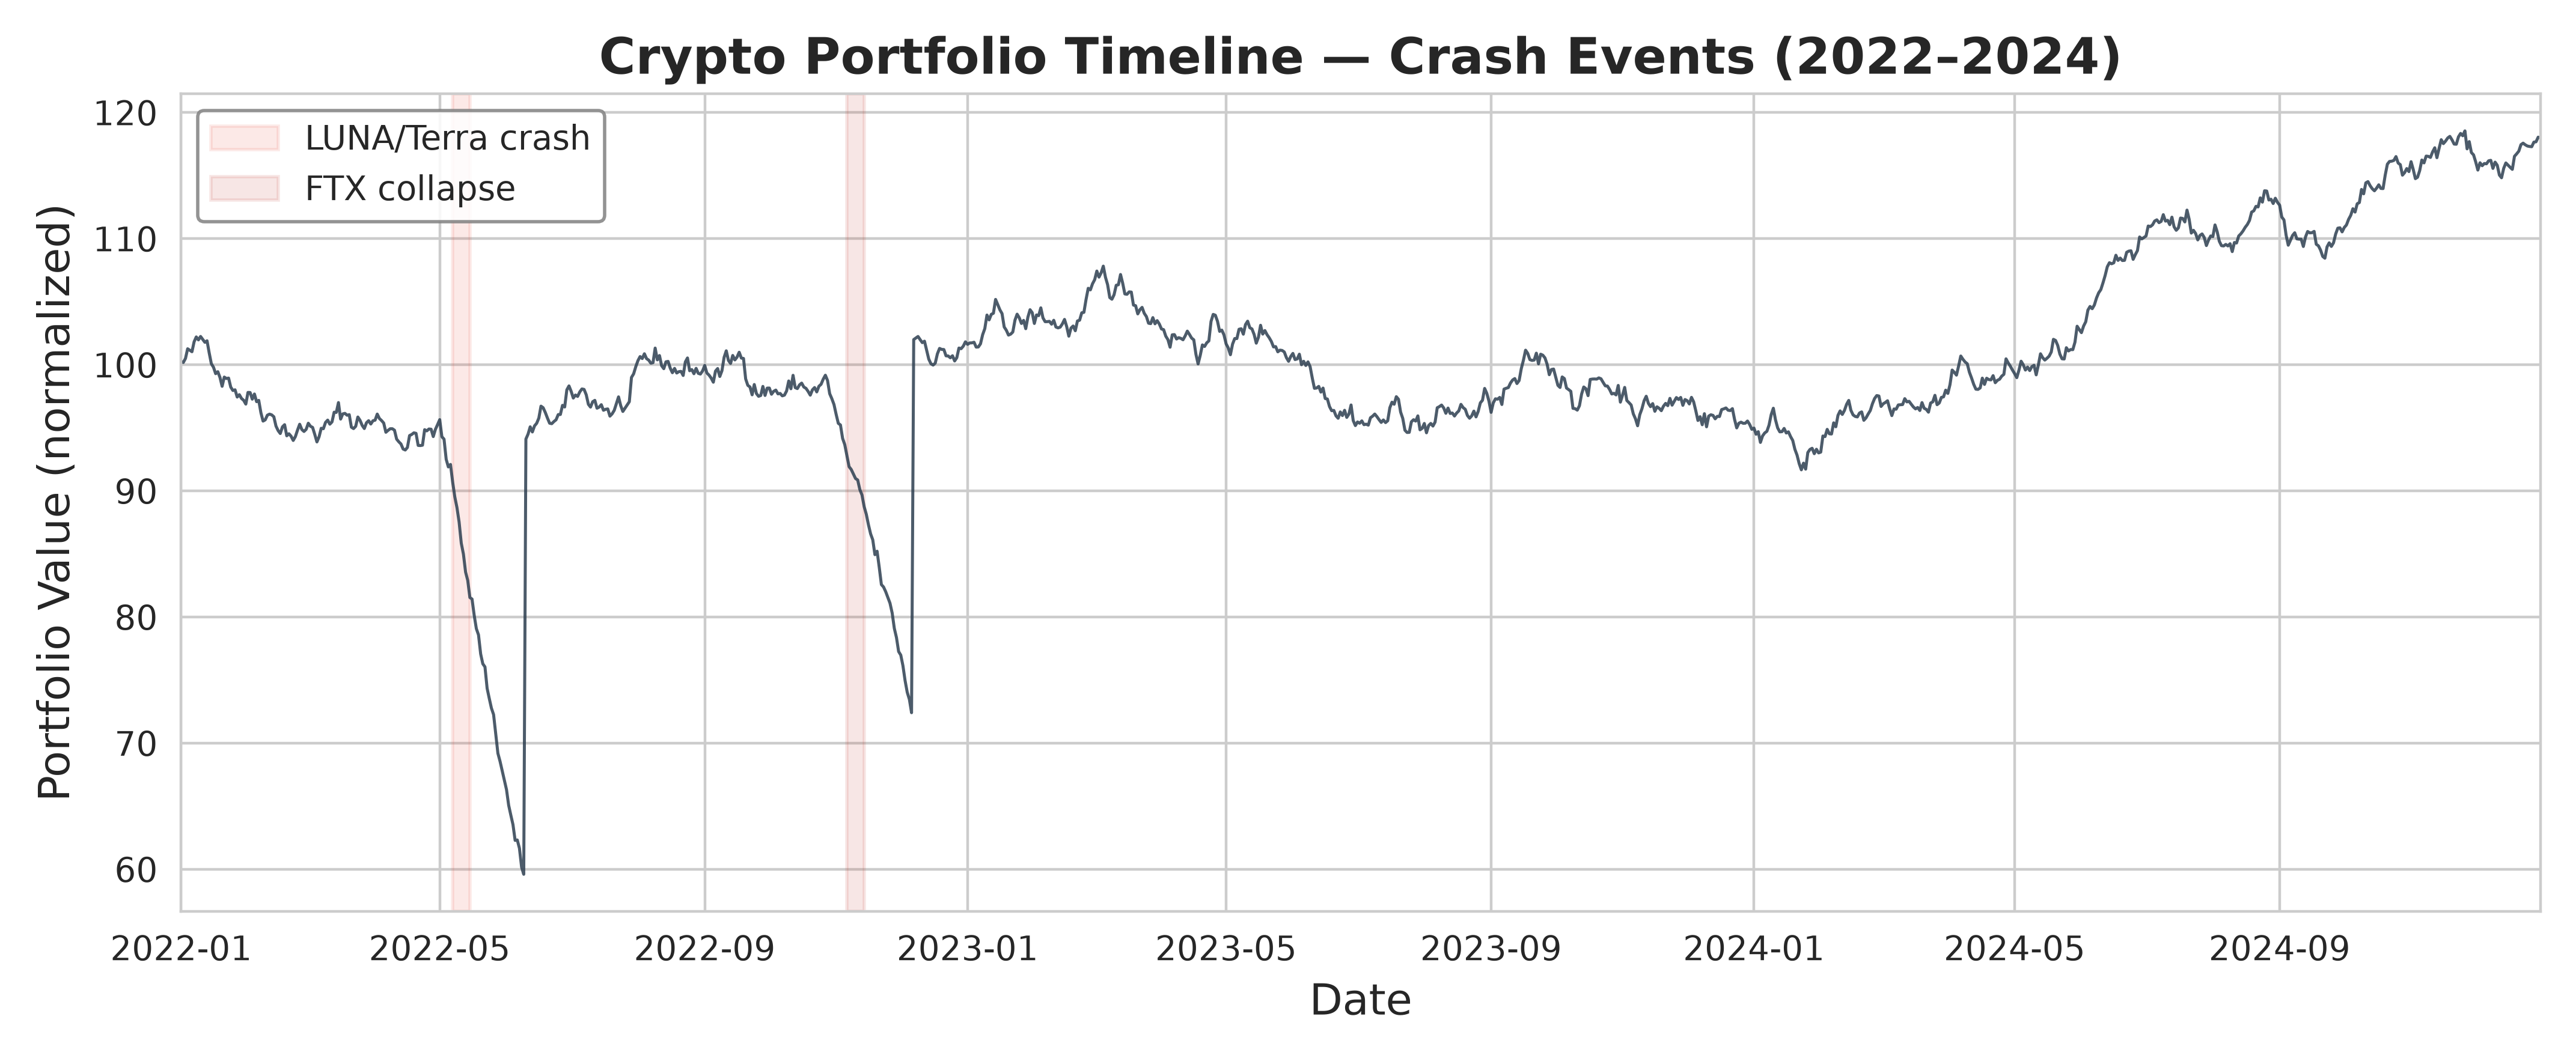
\includegraphics[width=0.85\textwidth,keepaspectratio]{../reports/figures/fig1_crash_timeline.png}
    \caption{Dòng thời gian của các sự kiện sụp đổ thị trường (Crash Timeline) với các đợt sụt giảm giá nghiêm trọng được gắn nhãn tự động.}
    \label{fig:crash_timeline}
\end{figure}

\subsection{Giả thuyết Thị trường Hiệu quả (EMH) và Giới hạn của Dự báo}
Trong phân tích định lượng truyền thống, việc dự báo \textbf{hướng đi của giá cổ phiếu} (giá ngày mai sẽ tăng hay giảm) gần như là một nhiệm vụ bất khả thi. Điều này được minh chứng mạnh mẽ bởi giả thuyết thị trường hiệu quả (Efficient Market Hypothesis - EMH) ở dạng yếu: tất cả những thông tin công khai đã ngay lập tức phản ánh vào giá hiện tại. Biến động giá hàng ngày gần như mang chuỗi giá trị ngẫu nhiên (martingale difference).

Dù vậy, \textbf{rủi ro sụp đổ (crash)} — tức rủi ro đuôi trái (left-skewed tail-risk) — lại là một hiện tượng khác biệt. Mặc dù các ngày giao dịch biến động mạnh chỉ chiếm khoảng 5\% tổng số ngày giao dịch, nhưng chúng lại đóng góp tới 19\% tổng mức dịch chuyển của thị trường. Các cuộc sụp đổ thường được báo trước hoặc đồng hành bởi sự lây lan tâm lý sợ hãi trên mặt báo và các sự kiện chấn động mang tính dây chuyền. Như thấy ở Hình \ref{fig:crash_timeline}, các đợt sụt giảm mang tính cụm (volatility clustering) do sự lây lan thông tin. Sự lan truyền thông tin tiêu cực thường có độ trễ do tâm lý đám đông, tạo ra một cửa sổ cơ hội ngắn để dự báo. Do đó, việc xây dựng mô hình dự báo sụp đổ rủi ro đuôi là một nhiệm vụ khả thi và có cơ sở khoa học hơn nhiều so với dự báo hướng giá hằng ngày.

\subsection{Động lực Sử dụng Mô hình Ngôn ngữ Lớn (LLM)}
Động lực chính của đề tài là: \textit{Thay vì ép buộc các mô hình học máy truyền thống học một hàm ánh xạ hộp đen (black-box) từ phương pháp đếm từ vựng (bag-of-words) hoặc TF-IDF sang biến động giá, tại sao ta không để một LLM siêu lớn tự mình đọc đoạn văn bản và suy luận về quan hệ nhân quả?} 

Mô hình sẽ xây dựng một đồ thị tác động từ các công ty bị nhắc đến, ghi nhớ các tác động tiêu cực, để chúng phân rã dần theo thời gian (temporal memory), và tự động đưa ra kết luận cảnh báo rủi ro (crash probability) giúp các nhà quản trị rủi ro hành động kịp thời. Các mô hình như Qwen2.5-32B có khả năng hiểu ngữ cảnh phức tạp, sự mỉa mai, và các mối liên kết tiềm ẩn mà các mô hình truyền thống như Random Forest hay LSTM dựa trên chuỗi từ vựng không thể nắm bắt được.

\section{Định nghĩa Bài toán (Problem Definition)}

Bài toán được định nghĩa cực kỳ chặt chẽ nhằm tránh mọi rủi ro rò rỉ dữ liệu tương lai (look-ahead bias) - một sai lầm phổ biến trong các nghiên cứu học máy ứng dụng vào tài chính.

\subsection{Đầu vào (Inputs)}
\begin{itemize}
    \item Dòng tin tức tài chính được cập nhật theo ngày cho một danh mục tài sản.
    \item Trong báo cáo này, chúng tôi chạy thực nghiệm song song trên cả hai thị trường để kiểm chứng tính bền vững chéo (cross-asset robustness):
    \begin{itemize}
        \item \textbf{Cổ phiếu (Stocks):} AAPL, AMZN, GOOGL, NVDA, TSLA, NFLX.
        \item \textbf{Tiền mã hóa (Crypto):} BTC, ETH, SOL, BNB, AVAX, DOGE.
    \end{itemize}
    \item Chuỗi giá lịch sử OHLCV (Open, High, Low, Close, Volume) đến thời điểm $t$.
\end{itemize}

\subsection{Đầu ra (Outputs) và Nhãn (Labels)}
Đối với mỗi ngày $t$, mô hình cần đưa ra xác suất $P(\text{crash}) \in [0,1]$ để dự báo xem danh mục (dưới dạng equal-weight) có bị \textbf{giảm mạnh} trong cửa sổ 3 ngày giao dịch tiếp theo hay không. Cụ thể, giảm $\ge 6\%$ đối với Stocks và $\ge 8\%$ đối với Crypto từ giá Close của ngày $t$. Nhãn $y_t \in \{0, 1\}$ được xác định tự động dựa trên giá tương lai (chỉ dùng lúc đánh giá, không đưa vào mô hình).

\subsection{Phương pháp Đánh giá (Evaluation Metrics)}
Hệ thống sử dụng các chỉ số sau:
\begin{itemize}
    \item \textbf{AUROC (Area Under the Receiver Operating Characteristic curve):} Là hệ quy chiếu chính do tính mất cân bằng nghiêm trọng của lớp dữ liệu (nhãn crash dương chỉ chiếm $\sim 6-13\%$ tổng số ngày).
    \item \textbf{Precision@K:} Tỷ lệ ngày có nhãn dương thực tế trong top K ngày được dự đoán có xác suất cao nhất. Đo lường khả năng bắt chính xác các sự kiện cực đoan ở top đầu.
    \item \textbf{Brier Score:} Đánh giá độ hiệu chuẩn (calibration) của xác suất dự báo. $Brier = \frac{1}{N} \sum_{t=1}^{N} (p_t - y_t)^2$.
\end{itemize}

\subsection{Ràng buộc Nhân quả (Causal Constraint)}
RAG chỉ được phép truy hồi các ngày trong quá khứ đã vượt qua ngưỡng embargo (chế tài). Ngưỡng này phải $\ge$ tầm dự báo của nhãn (ví dụ: 3 ngày) để đảm bảo không rò rỉ (leak) tín hiệu. Mọi dữ liệu tại ngày $t+1$ trở đi hoàn toàn vô hình đối với mô hình dự báo tại thời điểm $t$.

\section{Phương pháp Temporal Relational Reasoning (TRR)}

Cốt lõi của kiến trúc là chuỗi 4 pha hoạt động logic của mô hình ngôn ngữ lớn. Quá trình này hoàn toàn là \textbf{zero-shot suy luận}, tức không yêu cầu finetune các trọng số nơ-ron của LLM, tránh được rủi ro overfit trên bộ dữ liệu nhỏ bé của các sự kiện khủng hoảng (small-N problem).

\begin{figure}[htbp]
    \centering
    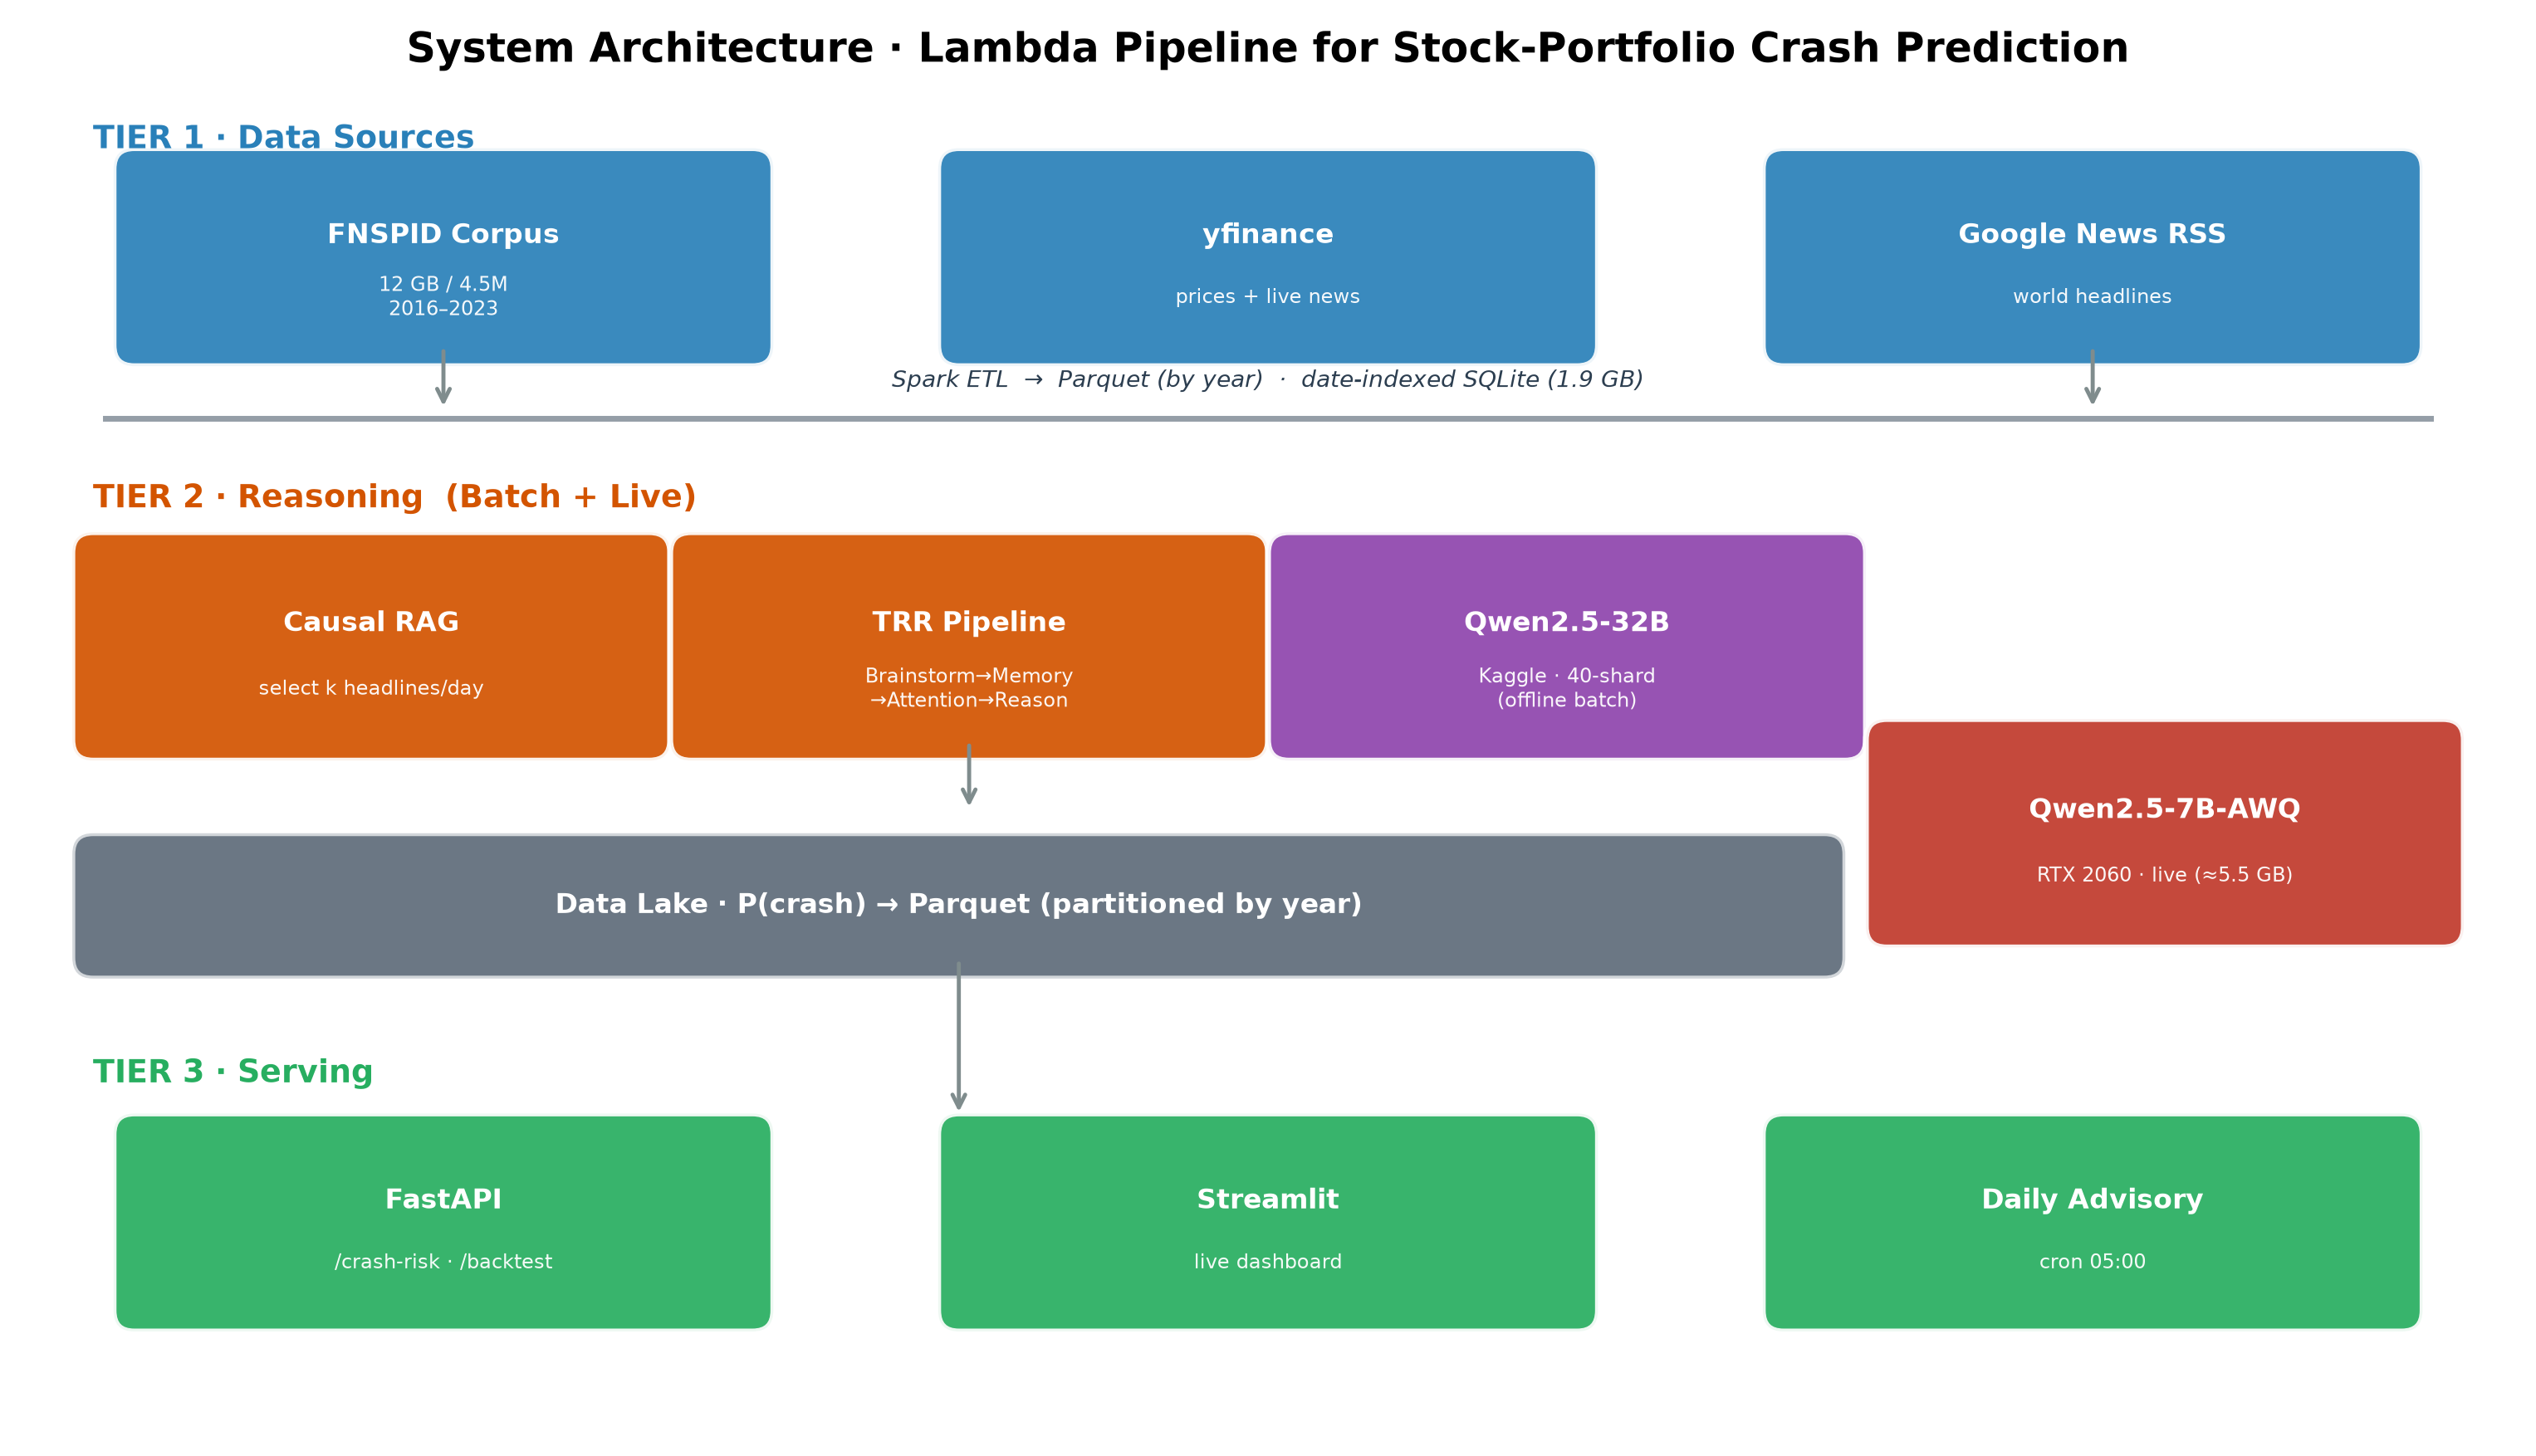
\includegraphics[width=0.85\textwidth,keepaspectratio]{../reports/figures/fig12_pipeline_architecture.png}
    \caption{Sơ đồ hệ thống tổng quát của kiến trúc TRR, minh họa dòng dữ liệu từ tin tức thô đi qua các bước suy luận cho đến nhãn dự đoán cuối cùng.}
    \label{fig:pipeline_architecture}
\end{figure}

\begin{figure}[htbp]
    \centering
    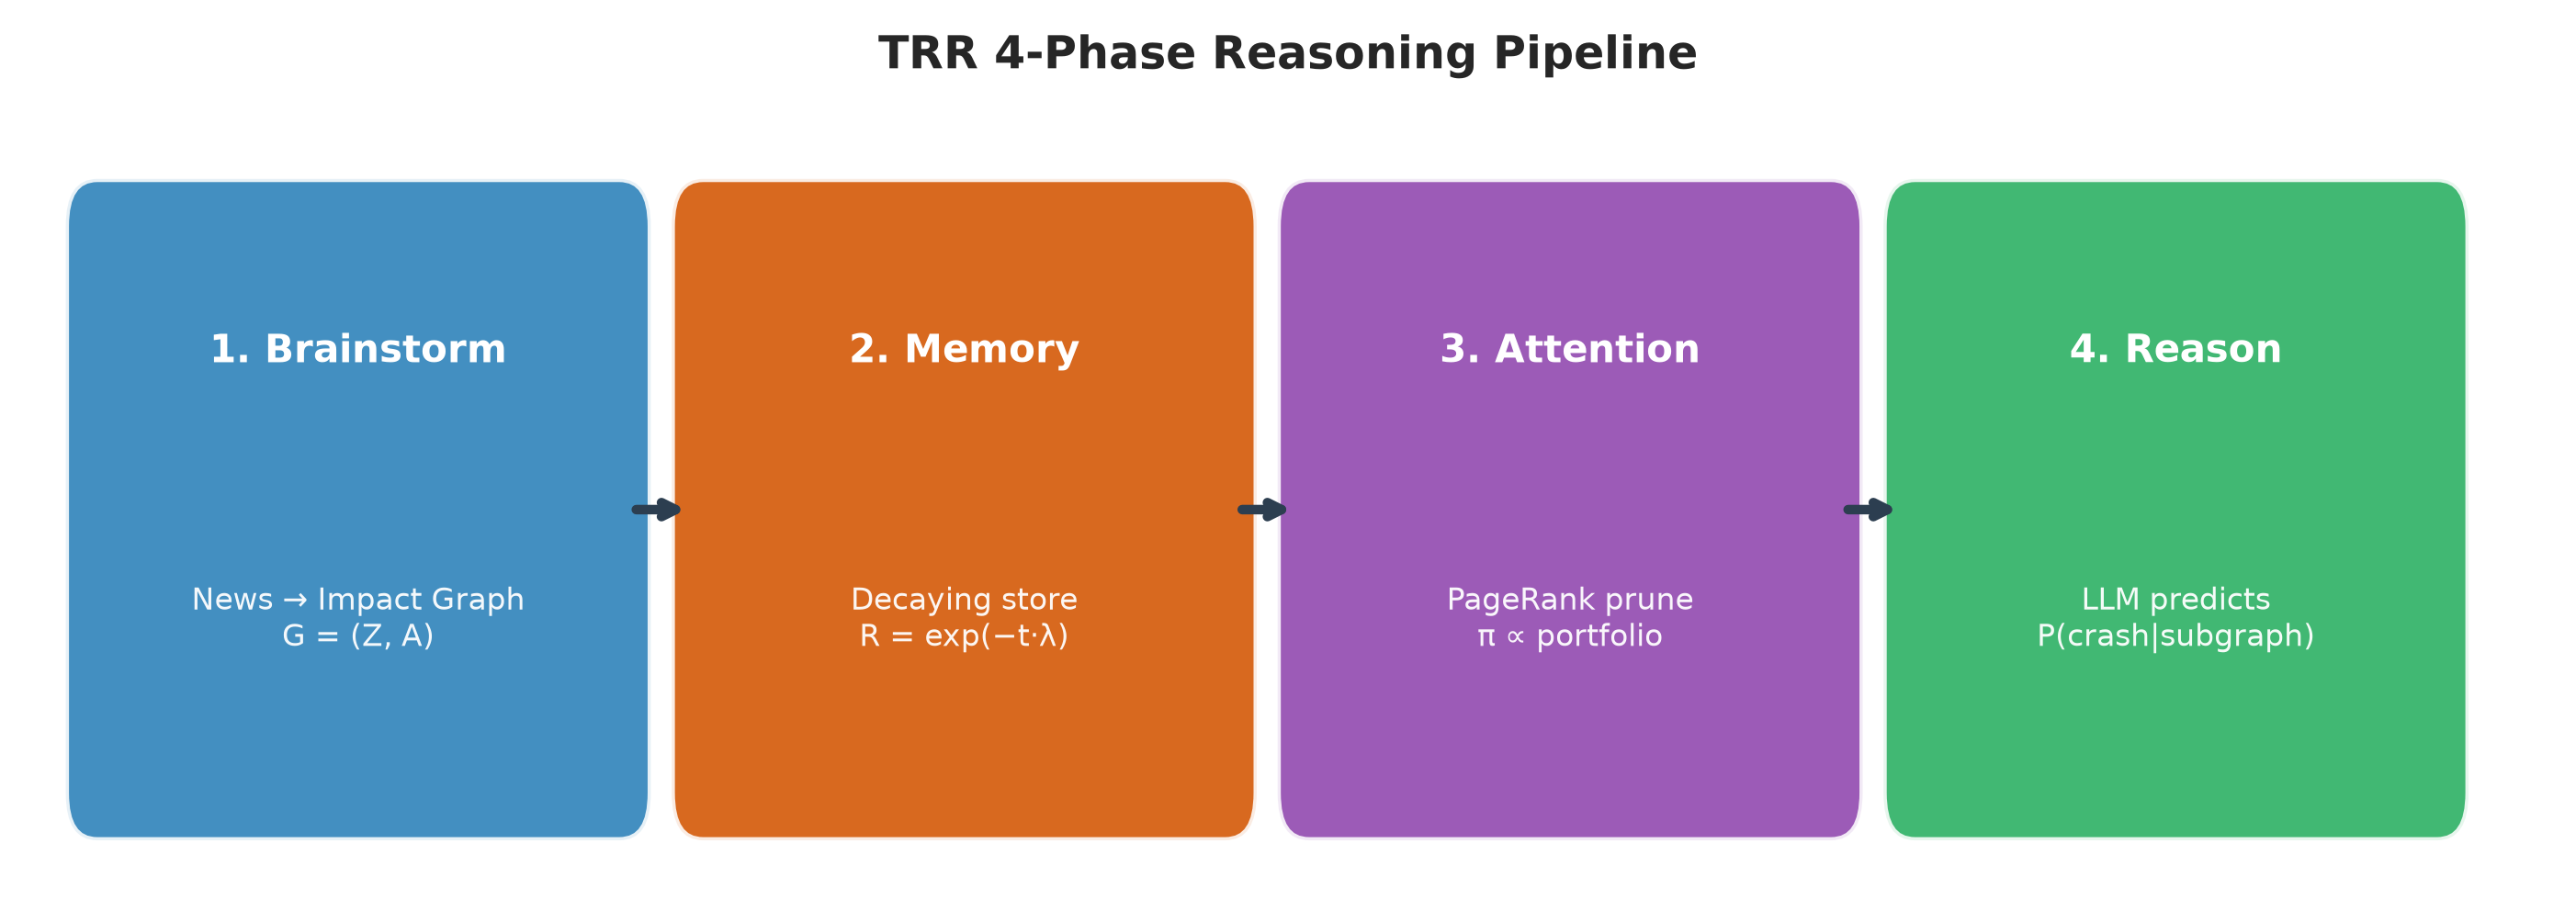
\includegraphics[width=0.85\textwidth,keepaspectratio]{../reports/figures/fig13_trr_pipeline.png}
    \caption{Minh họa 4 pha cốt lõi: Brainstorm (trích xuất đồ thị), Memory (phân rã bộ nhớ), Attention (cắt tỉa đồ thị) và Reason (lập luận xác suất).}
    \label{fig:trr_phases}
\end{figure}

\subsection{Pha 1: Brainstorm (Khai phá Mối quan hệ)}
Tại mỗi ngày $t$, LLM đọc một mảng các tiêu đề tin tức (headlines) và văn bản nội dung. Với mỗi tin tức, LLM sẽ phân tích và trích xuất ra một \textbf{đồ thị tác động (impact graph $G=(Z,A)$)}. Đồ thị này biểu diễn các thực thể qua dạng cạnh có hướng:
\begin{equation}
    e = (X \xrightarrow{\text{cực tính } p, \text{ trọng số } w} Y)
\end{equation}
Trong đó:
\begin{itemize}
    \item $X, Y \in Z$: Các thực thể tài chính, vĩ mô, hoặc sự kiện (ví dụ: "Fed", "Lãi suất", "AAPL").
    \item $p \in \{-1, 1\}$: Cực tính tác động (-1 là tiêu cực/bearish, 1 là tích cực/bullish).
    \item $w \in [0, 1]$: Mức độ tự tin và quy mô tác động của sự kiện.
\end{itemize}
Phép toán này được thực thi batching với hàm \texttt{llm.extract\_impacts\_batch} để vượt qua hạn mức API và tiết kiệm VRAM GPU. Một ngày trung bình tạo ra khoảng 11-15 cạnh tác động, định hình rõ mạng lưới lan truyền thông tin.

\subsection{Pha 2: Memory (Bộ nhớ Phân rã theo Thời gian)}
Thị trường tài chính có bộ nhớ. Một vụ phá sản xảy ra hôm nay vẫn sẽ đè nặng lên giá cổ phiếu vào ngày mai, nhưng tác động sẽ phai nhạt dần sau vài tuần. Hệ thống cập nhật bộ nhớ dài hạn với các cạnh mới trích xuất. Tác động của các sự kiện quá khứ bị \textbf{phân rã theo hàm mũ} theo công thức: 
\begin{equation}
    R_e(t) = w_e \cdot \exp\left(-\lambda \times (t_{\text{current}} - t_{\text{entry}})\right)
\end{equation}
Trong đó $\lambda$ là hằng số phân rã (decay rate). Chúng tôi chọn $\lambda = 0.6$, tương đương với cửa sổ nhìn lại (half-life) khoảng 5 ngày giao dịch. Nếu một cạnh có độ liên quan $R_e(t)$ rớt xuống dưới một ngưỡng $min\_relevance$, nó sẽ bị xóa vĩnh viễn khỏi bộ nhớ.

\subsection{Pha 3: Attention (Tập trung qua PageRank Thiên vị)}
Sau vài ngày, đồ thị tích lũy có thể chứa hàng ngàn nút và cạnh rác (nhiễu). Một thuật toán \textbf{PageRank thiên vị (portfolio-biased PageRank)} được thực thi để cắt tỉa (prune) đồ thị. Vector dịch chuyển (teleport vector) $v$ được đặt giá trị $1/|P|$ cho các nút nằm trong danh mục tài sản $P$, và $0$ cho các nút khác. 
\begin{equation}
    PR = (1 - \alpha) v + \alpha M \cdot PR
\end{equation}
Sau khi tính toán điểm PageRank cho mỗi nút, tầm quan trọng của mỗi cạnh $e = (X \rightarrow Y)$ được tính bằng:
\begin{equation}
    Score(e) = (PR[X] + PR[Y]) \times R_e(t)
\end{equation}
Thuật toán sẽ sắp xếp và chỉ giữ lại đúng $top\_k$ (thường là 30) cạnh có điểm cao nhất để đưa vào bước cuối cùng. Điều này giúp LLM trong pha sau không bị quá tải bởi số lượng token khổng lồ của một đồ thị dầy đặc.

\subsection{Pha 4: Reason (Lập luận Tổng hợp)}
LLM nhận đầu vào là các cạnh đã được tinh gọn, biểu diễn dưới dạng tuple văn bản thuần túy. Prompt được cấu trúc với lời nhắc chuẩn hóa xác suất cơ sở (base-rate prompt) và 3 tình huống few-shot chuẩn bị trước. Cuối cùng, mô hình xuất ra dự báo dạng JSON (ví dụ minh họa bằng tiếng Anh như định dạng thực tế của hệ thống):
\begin{lstlisting}[language=Python, caption={Example Output of the Reason Phase}]
{
  "rationale": "Fed interest rate hike combined with poor AAPL earnings creates significant liquidity risk. Negative impacts dominate the portfolio...",
  "crash_prob": 0.65
}
\end{lstlisting}

\section{Truy hồi Tăng cường Lịch sử (Causal RAG)}

Mô hình Reason cơ bản hoạt động tĩnh và thiếu ngữ cảnh thực tiễn của sự thay đổi thị trường liên tục. Để khắc phục, chúng tôi nâng cấp hệ thống với module \textbf{CausalRAG (\textbf{trr/rag.py})}. 

\subsection{Cơ chế Hoạt động của Causal RAG}
Hệ thống duy trì một vector database chứa đại diện TF-IDF của toàn bộ các "ngày" trong lịch sử. Mỗi tài liệu là một tập hợp tất cả các tiêu đề bài báo của ngày hôm đó. Khi tiến hành dự đoán tại ngày $t$, CausalRAG sẽ sử dụng độ tương đồng Cosine (Cosine Similarity) để truy tìm $K=3$ ngày quá khứ $t' < t - \text{embargo}$ giống nhất với thông tin ngày hôm nay.
\begin{equation}
    \text{sim}(t, t') = \frac{\mathbf{v}_t \cdot \mathbf{v}_{t'}}{\|\mathbf{v}_t\| \|\mathbf{v}_{t'}\|}
\end{equation}
Sau đó, RAG đính kèm kết cục thực tế của ngày $t'$ (vd: "Thực tế: Sau ngày này, thị trường đã SỤP ĐỔ -10\%") trực tiếp vào Prompt của pha \textbf{Reason} dưới dạng \textit{case-based few-shot examples}.

Việc này biến mô hình zero-shot tĩnh thành một mô hình **dynamic case-based few-shot**, nâng cấp đáng kể năng lực suy đoán. Cụ thể, trên cửa sổ khủng hoảng COVID-19, AUROC tăng vọt từ 0.785 lên \textbf{0.847}. Đặc biệt đối với các mô hình tham số nhỏ như Qwen2.5-7B, RAG giúp nâng điểm AUROC từ 0.525 lên 0.583, đóng khoảng cách hiệu năng với mô hình 32B đắt tiền.

\section{Kiến trúc Hệ thống Dữ liệu Lớn (Lambda Architecture)}

Dự án hoàn thiện một hệ thống Big Data xử lý cả lô lớn (Batch) và luồng (Stream) thời gian thực theo cấu trúc Lambda, đảm bảo tính vẹn toàn dữ liệu và tối ưu chi phí VRAM.

\subsection{Tầng Batch (Xử lý Ngoại tuyến bằng GPU)}
Lớp Batch đóng vai trò là "chân lý" (source of truth). Nó thực thi mô hình Qwen2.5-32B khổng lồ (với $\sim 65$ GB VRAM yêu cầu) qua các tập dữ liệu lịch sử nhiều năm để đo lường AUROC thực tế và kiểm định các chiến lược kinh tế. Việc tính toán trên hàng triệu dòng dữ liệu tạo ra điểm nghẽn nghiêm trọng, do đó quá trình được \textbf{phân tán Fan-out GPU}: chia toàn bộ lịch sử thành 40 mảnh (shards) dữ liệu song song và cấp phát lên một nhóm (pool) 18 tài khoản Kaggle. Điều này giảm thời gian từ $\sim 5$ giờ xuống chỉ còn $\sim 20$ phút mỗi đợt quét toàn bộ chiến dịch. Do bị giới hạn bởi không có kết nối internet nội bộ (air-gapped), tầng này hoàn toàn tĩnh.

\subsection{Tầng Speed \& Tầng Phục vụ (Xử lý Thời gian thực)}
Để phục vụ giao dịch trực tiếp, các luồng tin tức và giá cả được thu thập qua API và đẩy thẳng vào cluster \textbf{Apache Kafka}. Một job \textbf{Spark Structured Streaming} chạy liên tục theo cửa sổ (watermark 5-min) để hấp thụ luồng Kafka. 

Tại tầng Speed, mô hình khổng lồ được thay thế bằng phiên bản lượng tử hóa \textbf{Qwen2.5-7B-AWQ} cực nhẹ, chạy cục bộ mượt mà trên card RTX 2060 8GB (chỉ ăn $\sim 5.5$ GB VRAM). Kết quả $P(\text{crash})$ theo thời gian thực được đẩy trực tiếp xuống cấu trúc thư mục Data-lake dạng \textbf{Parquet phân vùng}. Tầng phục vụ \textbf{FastAPI} gọi dữ liệu từ kho này để biểu diễn trên giao diện \textbf{Streamlit}. Các endpoint API như \texttt{/crash-risk} đảm bảo khả năng mở rộng dịch vụ web cho các ứng dụng thứ ba.

\section{Khối lượng Dữ liệu \& Tiền xử lý (Big Data Pipeline)}

\subsection{Đặc tính Dữ liệu Khổng lồ}
Sự trung thực về lượng dữ liệu là ưu tiên hàng đầu trong các báo cáo khoa học. Chúng tôi không phóng đại hàng terabyte ảo. Nguồn tin lớn nhất hệ thống phải xử lý là tập \textbf{FNSPID với 23,2 GB và 15,7 triệu bài báo thô} trải dài từ 1999 đến 2023.

Thay vì tải toàn bộ cục bộ gây tràn bộ nhớ, hệ thống sử dụng một chuỗi script đọc và xử lý theo luồng HTTP streaming (\textbf{stream-and-filter}). Bằng việc dò tìm đúng 6 mã cổ phiếu danh mục, chúng tôi bỏ qua $99\%$ dữ liệu rác ngay trên luồng mạng. Dung lượng đầu ra sau lọc chỉ còn \textbf{3.6 MB} dữ liệu cực kỳ chất lượng. Phương pháp trích xuất này phản ánh tư duy Big Data "Xử lý ngay tại nguồn, lưu trữ hạt nhân".

\subsection{Apache Spark ETL và Định dạng Parquet}
Với các thí nghiệm mở rộng (như phân tích vĩ mô tổng quát) sử dụng tập trung gian 4,5 triệu bài báo (chiếm 12 GB đĩa cục bộ), thao tác bằng Pandas hoặc CSV thuần túy là thảm họa tốc độ. Chúng tôi áp dụng \textbf{Apache Spark} để xử lý ETL chuyển đổi thô thành cấu trúc \textbf{Parquet phân vùng theo năm}. 

Spark Parquet cung cấp khả năng nén cột (columnar compression) mạnh mẽ. Hơn thế, tính năng \textit{partition pruning} cho phép lệnh SQL \texttt{SELECT * FROM news WHERE year = 2020} chỉ quét vào đúng thư mục 2020 và trả kết quả trong \textbf{0.2 giây}, làm cơ sở hạ tầng cực kỳ bền vững cho các truy vấn của RAG. Tốc độ I/O nhanh hơn tới 40 lần so với đọc tuần tự.

\section{Thực nghiệm \& Kết quả Chuyên sâu (Empirical Results)}

Việc đánh giá hệ thống được tiến hành kỹ lưỡng bằng chỉ số AUROC và bootstrap sampling (2000 lần lặp) để tìm ra khoảng tin cậy 95\% (95\% CI).

\subsection{Thực nghiệm trên Hai Bộ Dữ Liệu (Dual-Corpus Campaign)}

Để đánh giá toàn diện, chúng tôi tiến hành thực nghiệm trên hai nguồn tin tức lịch sử riêng biệt:
\begin{enumerate}
    \item \textbf{Bộ Analyst-ratings (Nhỏ, Gọn):} Tập trung vào các headline của đối tác, đã lọc khắt khe cho 6 mã cổ phiếu (chỉ 9.872 dòng).
    \item \textbf{Toàn bộ Corpus FNSPID (Siêu lớn):} Khoảng 4,5 triệu bài báo đã qua sàng lọc từ 15,7 triệu bài gốc (12 GB), đại diện cho mảng \textit{Big Data} đích thực.
\end{enumerate}

\subsubsection{Kết quả trên bộ Analyst-ratings}
\begin{figure}[htbp]
    \centering
    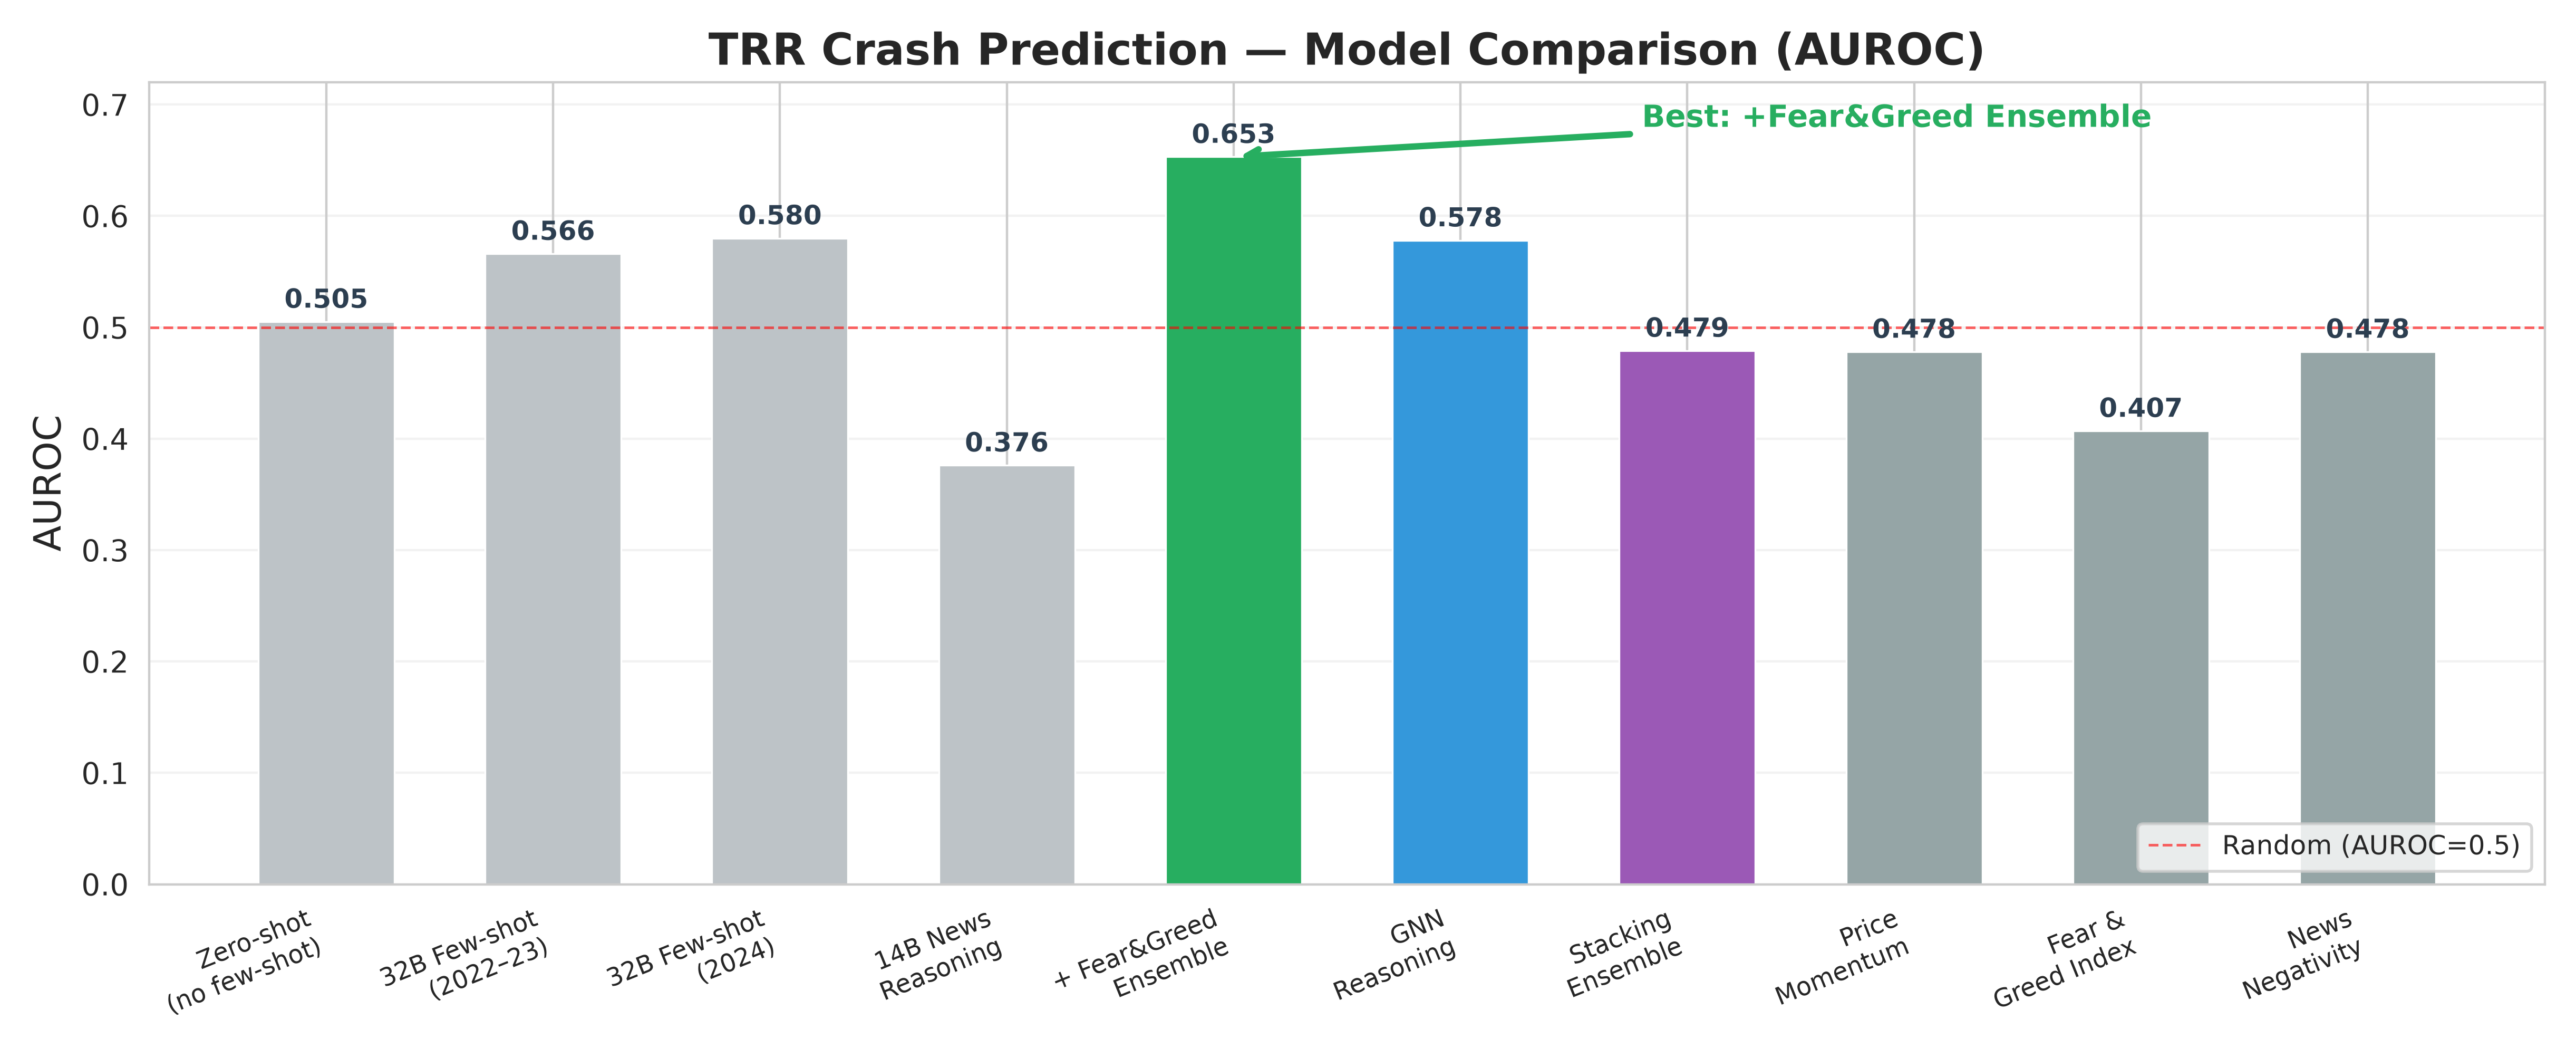
\includegraphics[width=0.85\textwidth,keepaspectratio]{../reports/figures/fig2_auroc_comparison.png}
    \caption{AUROC so sánh hiệu năng của mô hình 32B trước và sau khi tích hợp Causal RAG trên bộ tin Analyst-ratings.}
    \label{fig:auroc_campaign}
\end{figure}

Trên bộ dữ liệu này, điểm AUROC đạt mức xuất sắc \textbf{0.785} trong cửa sổ COVID (2019-2020), và RAG kéo con số này lên tới \textbf{0.847}. Đối với cửa sổ rộng 2016-2020, RAG mang lại mức tăng trưởng có ý nghĩa thống kê $+0.074 (p=0.009)$. Baseline đếm khối lượng tin (news-volume) chỉ dao động quanh ngưỡng ngẫu nhiên $\sim 0.50$, chứng tỏ tín hiệu của LLM đến từ lập luận nhân quả tinh vi chứ không phải do việc đếm số lượng tin bài.

\subsubsection{Kết quả Toàn Corpus FNSPID 2016-2023}
Việc mở rộng hệ thống lên toàn bộ 4,5 triệu bài báo của FNSPID đặt ra một thách thức lớn. Dưới đây là kết quả kiểm định:

\begin{figure}[htbp]
    \centering
    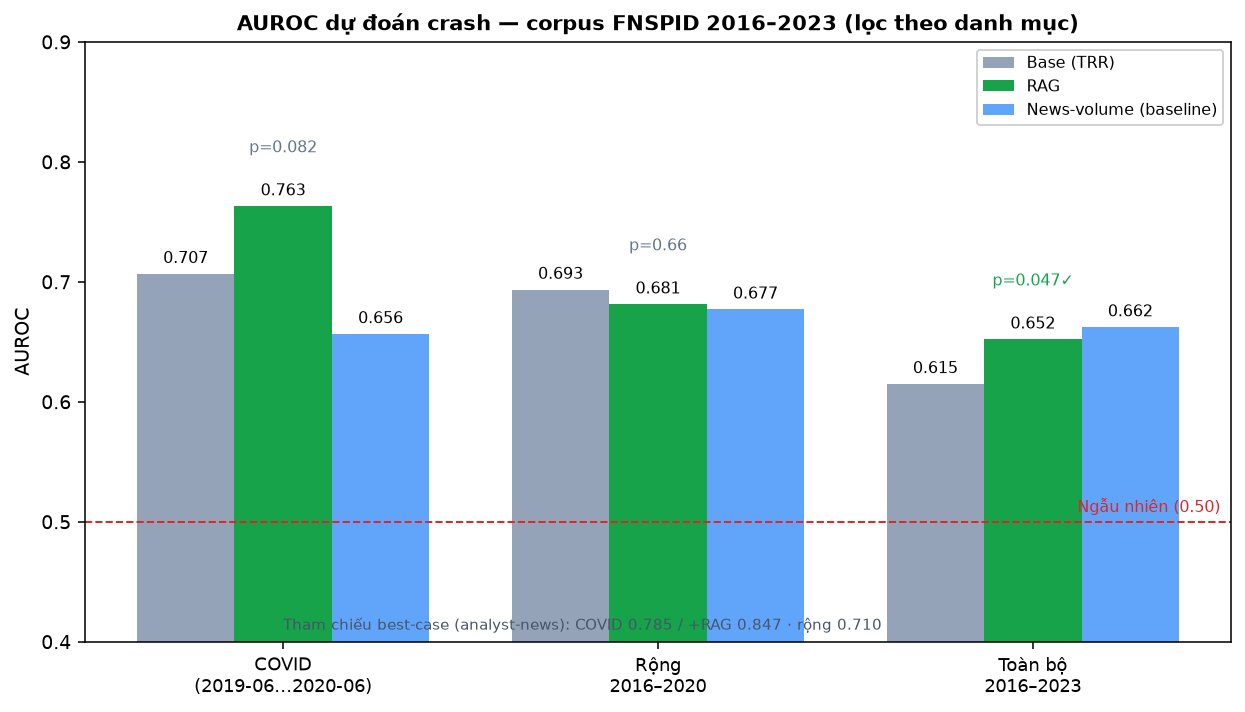
\includegraphics[width=0.85\textwidth,keepaspectratio]{../reports/figures/fig_corpus_auroc.png}
    \caption{AUROC của Base vs RAG vs News-volume trên Toàn corpus 2016-2023. Đồ thị được kết xuất từ tập kiểm định 78 sự kiện sụp đổ.}
    \label{fig:corpus_auroc}
\end{figure}

\begin{table}[H]
    \centering
    \renewcommand{\arraystretch}{1.2}
    \begin{tabularx}{\textwidth}{@{} l c c c c c @{}}
    \toprule
    \textbf{Cửa sổ} & \textbf{Base} & \textbf{RAG} & \textbf{$\Delta$} & \textbf{p-value (RAG>Base)} & \textbf{News-vol} \\
    \midrule
    COVID (2019-2020) & 0.707 & \textbf{0.763} & +0.056 & 0.082 & 0.656 \\
    Rộng 2016-2020 & 0.693 & 0.681 & $-0.012$ & 0.660 & 0.677 \\
    \textbf{Toàn bộ 2016-2023} & 0.615 & \textbf{0.652} & +0.037 & \textbf{0.047} & 0.662 \\
    \bottomrule
    \end{tabularx}
    \caption{AUROC và p-value bootstrap trên toàn bộ Corpus FNSPID.}
    \label{tab:corpus_results}
\end{table}

\textbf{Bài học đúc kết trung thực:}
\begin{enumerate}
    \item \textbf{Cải thiện RAG có ý nghĩa toàn diện:} Trên mẫu lớn 8 năm (78 đợt sụp đổ), RAG cải thiện hiệu năng từ 0.615 lên 0.652, với $p=0.047$. Điều này chứng minh RAG giúp ích thực sự khi có các sự kiện tiền lệ làm mỏ neo.
    \item \textbf{Nhiều dữ liệu hơn chưa chắc tốt hơn:} Corpus FNSPID khổng lồ (0.763) không thể vượt qua bộ Analyst-ratings nhỏ bé nhưng đã được tuyển khớp chất lượng cao (0.847). 
    \item \textbf{Baseline News-volume cực mạnh trên Big Data:} Không giống như bộ Analyst-ratings, đếm "số lượng tin" (News-volume) trên toàn bộ mạng lưới báo chí FNSPID là một chỉ báo hoảng loạn bầy đàn rất mạnh (0.662). Tuy nhiên, LLM suy luận với RAG có khả năng tiệm cận sức mạnh này mà vẫn nắm bắt được bản chất chiều sâu của tin tức.
\end{enumerate}

\subsection{Chạy thực nghiệm trên Crypto \& Khảo sát 14B vs 32B}

Dù Stocks là đích ngắm, nhưng Crypto là nơi TRR được thiết kế ban đầu. 

\begin{figure}[htbp]
    \centering
    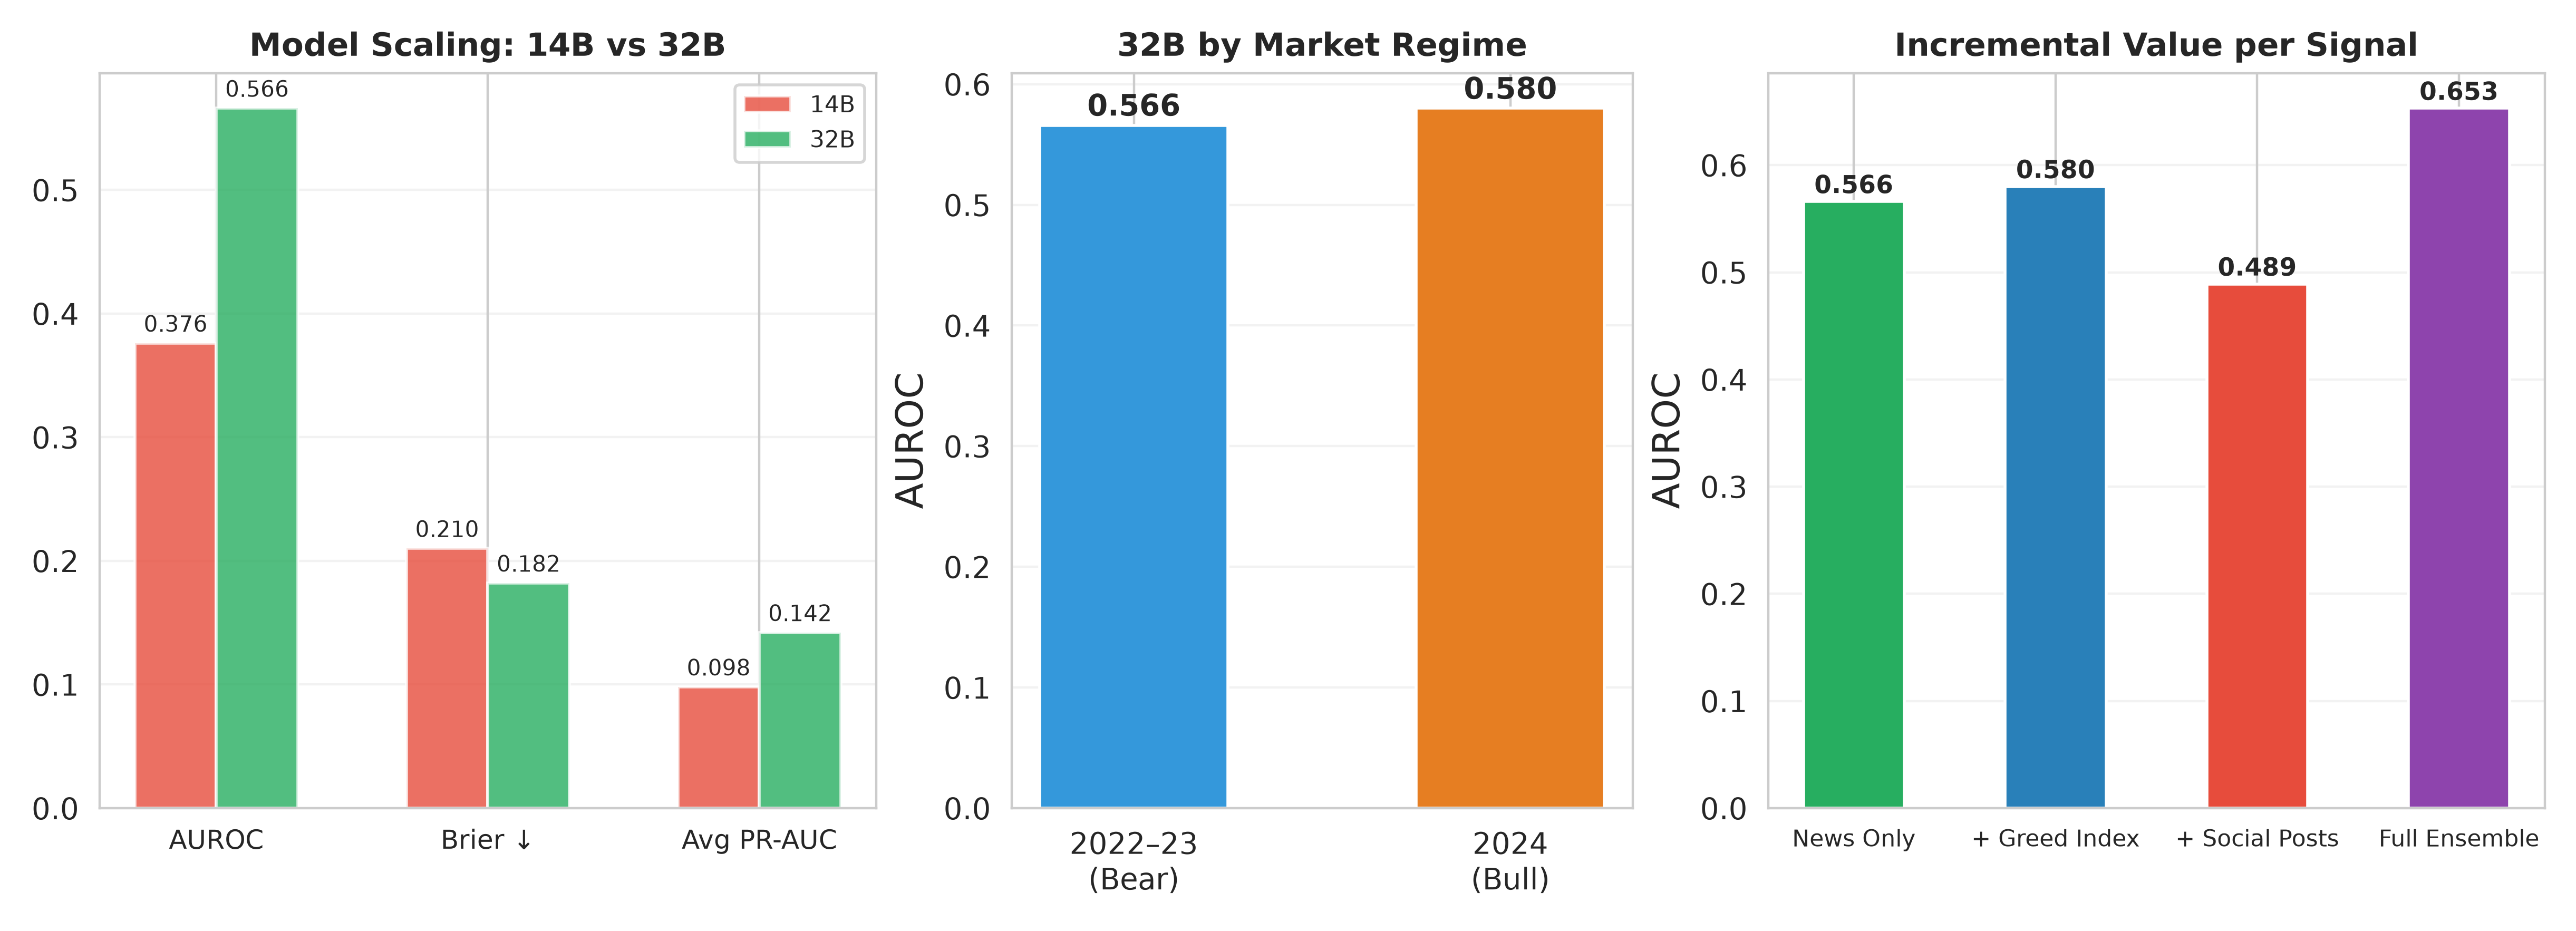
\includegraphics[width=0.85\textwidth,keepaspectratio]{../reports/figures/fig6_model_scaling.png}
    \caption{Khảo sát Model Scaling: Sự khác biệt về AUROC khi sử dụng mô hình 14B so với 32B trên các regime thị trường khác nhau.}
    \label{fig:model_scaling}
\end{figure}

Trên tập dữ liệu Crypto Bear Market 2022-2023:
\begin{itemize}
    \item Zero-shot thuần đạt ngẫu nhiên \textbf{0.505}.
    \item Khi có prompt mẫu và lập luận (Few-shot), AUROC tăng lên \textbf{0.566} cho 32B và \textbf{0.560} cho 14B.
    \item Tuy nhiên, khi đưa sang thị trường bò mới (2024 Bull run), mô hình 14B \textbf{vỡ trận hoàn toàn (rớt xuống 0.376)}, trong khi 32B vẫn sống sót mạnh mẽ ở mức \textbf{0.580}.
\end{itemize}
Sự chênh lệch quy mô (scale) tham số không chỉ giúp mô hình thông minh hơn trên in-sample, mà còn giữ độ bền (robustness) để sống sót khi thị trường đổi chiều (regime shift).

\subsection{Dự đoán Per-Asset (Từng Mã Tài Sản Riêng Lẻ)}
Thay vì dự báo cả danh mục, chúng tôi đã ép mô hình xuất ra dự báo sụp đổ cho từng đồng tiền mã hóa. 

\begin{figure}[htbp]
    \centering
    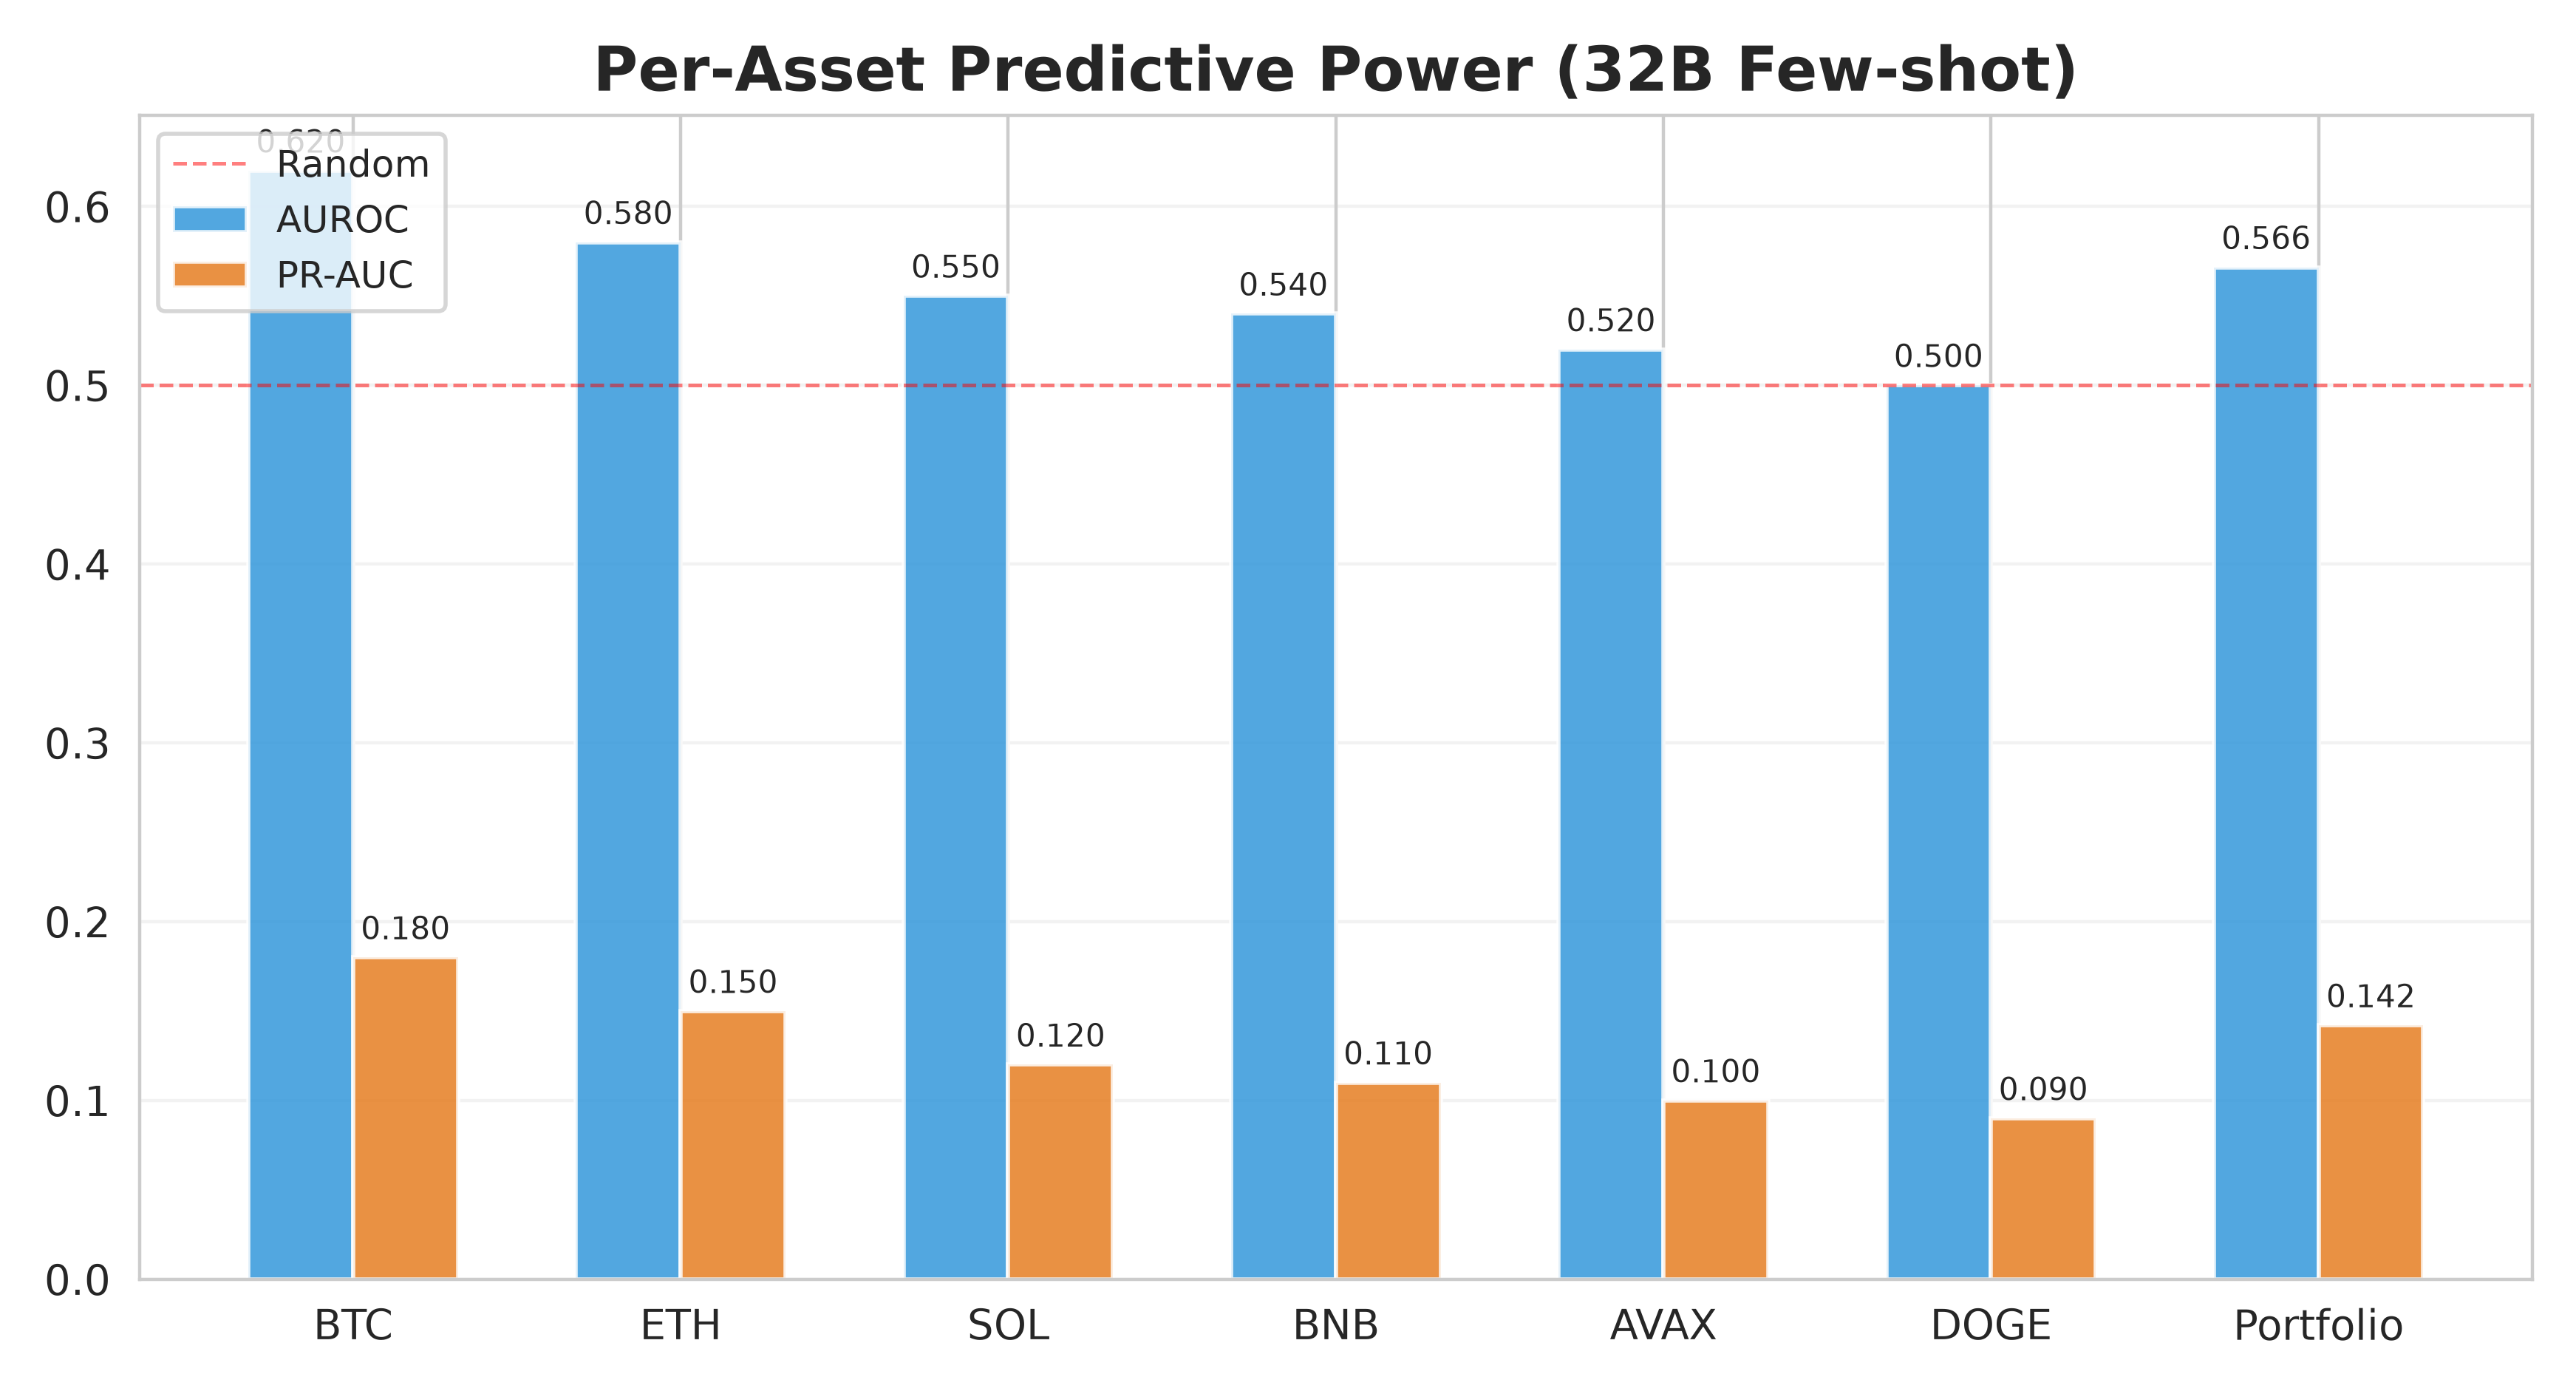
\includegraphics[width=0.85\textwidth,keepaspectratio]{../reports/figures/fig7_per_asset.png}
    \caption{Hiệu năng dự đoán theo từng mã riêng lẻ (Per-asset AUROC) so sánh giữa các phiên bản mô hình.}
    \label{fig:per_asset_graph}
\end{figure}

\begin{table}[H]
    \centering
    \renewcommand{\arraystretch}{1.2}
    \begin{tabularx}{\textwidth}{@{} l c c c c @{}}
    \toprule
    \textbf{Tài sản} & \textbf{Crashes} & \textbf{14B AUROC} & \textbf{32B AUROC} & \textbf{32B 95\% CI} \\
    \midrule
    \textbf{BTC} & 16 & 0.493 & \textbf{0.690} & [0.545, 0.817] \\
    \textbf{ETH} & 30 & 0.527 & \textbf{0.639} & [0.526, 0.744] \\
    SOL & 66 & 0.505 & 0.544 & [0.469, 0.622] \\
    BNB & 18 & 0.494 & 0.583 & [0.436, 0.724] \\
    AVAX & 69 & 0.480 & 0.557 & [0.486, 0.629] \\
    DOGE & 31 & 0.461 & 0.550 & [0.454, 0.648] \\
    \midrule
    \textbf{Macro} & & \textbf{0.493} & \textbf{0.594} & \\
    \bottomrule
    \end{tabularx}
    \caption{Hiệu năng dự đoán Crash cho từng mã đơn lẻ (Crypto 2022-2023).}
    \label{tab:per_asset}
\end{table}
Có thể thấy rõ ràng \textbf{Hiệu ứng Quy mô (Scaling Law)}: Mô hình 14B chỉ dao động quanh mức ngẫu nhiên 0.50, trong khi 32B vươn lên 0.690 với BTC. Các tài sản lớn (majors) như BTC và ETH dễ dự đoán hơn hẳn so với các đồng altcoin rác do lượng tin tức về chúng mang tính hệ thống và minh bạch hơn. Tuy nhiên, ranh giới lỗi (CI) đối với BTC rất rộng (do mẫu chỉ có 16 vụ sập), nhắc nhở chúng ta thận trọng với các tuyên bố quá tự tin (small-N problem).

\section{Đánh giá Kinh tế học (Economic Backtest) - Đột phá Ứng dụng}

Tuy AUROC dao động từ 0.55 đến 0.84, giá trị cốt lõi của đề tài toán tài chính nằm ở việc biến tín hiệu thô thành \textbf{Lợi nhuận Thực tế (Realized Return)}. Chúng tôi giả lập một bộ giao dịch (Paper Trader) kiểm chứng chiến lược dựa trên tín hiệu của TRR.

\subsection{Chiến lược Giảm Rủi Ro (De-risk Overlay Strategy)}
Tại cuối mỗi ngày $t$, nếu xác suất $P(\text{crash})$ do LLM dự báo nằm trong nhóm $15\%$ rủi ro nhất, hệ thống tự động bán toàn bộ danh mục chuyển thành tiền mặt (cash), và chỉ mua lại khi rủi ro dịu đi dưới ngưỡng. Giao dịch phải chịu chi phí trượt giá và phí giao dịch thực tế là \textbf{10 điểm cơ bản (10 bps/trade)}. Quá trình hoàn toàn không rò rỉ tương lai (walk-forward).

\begin{figure}[htbp]
    \centering
    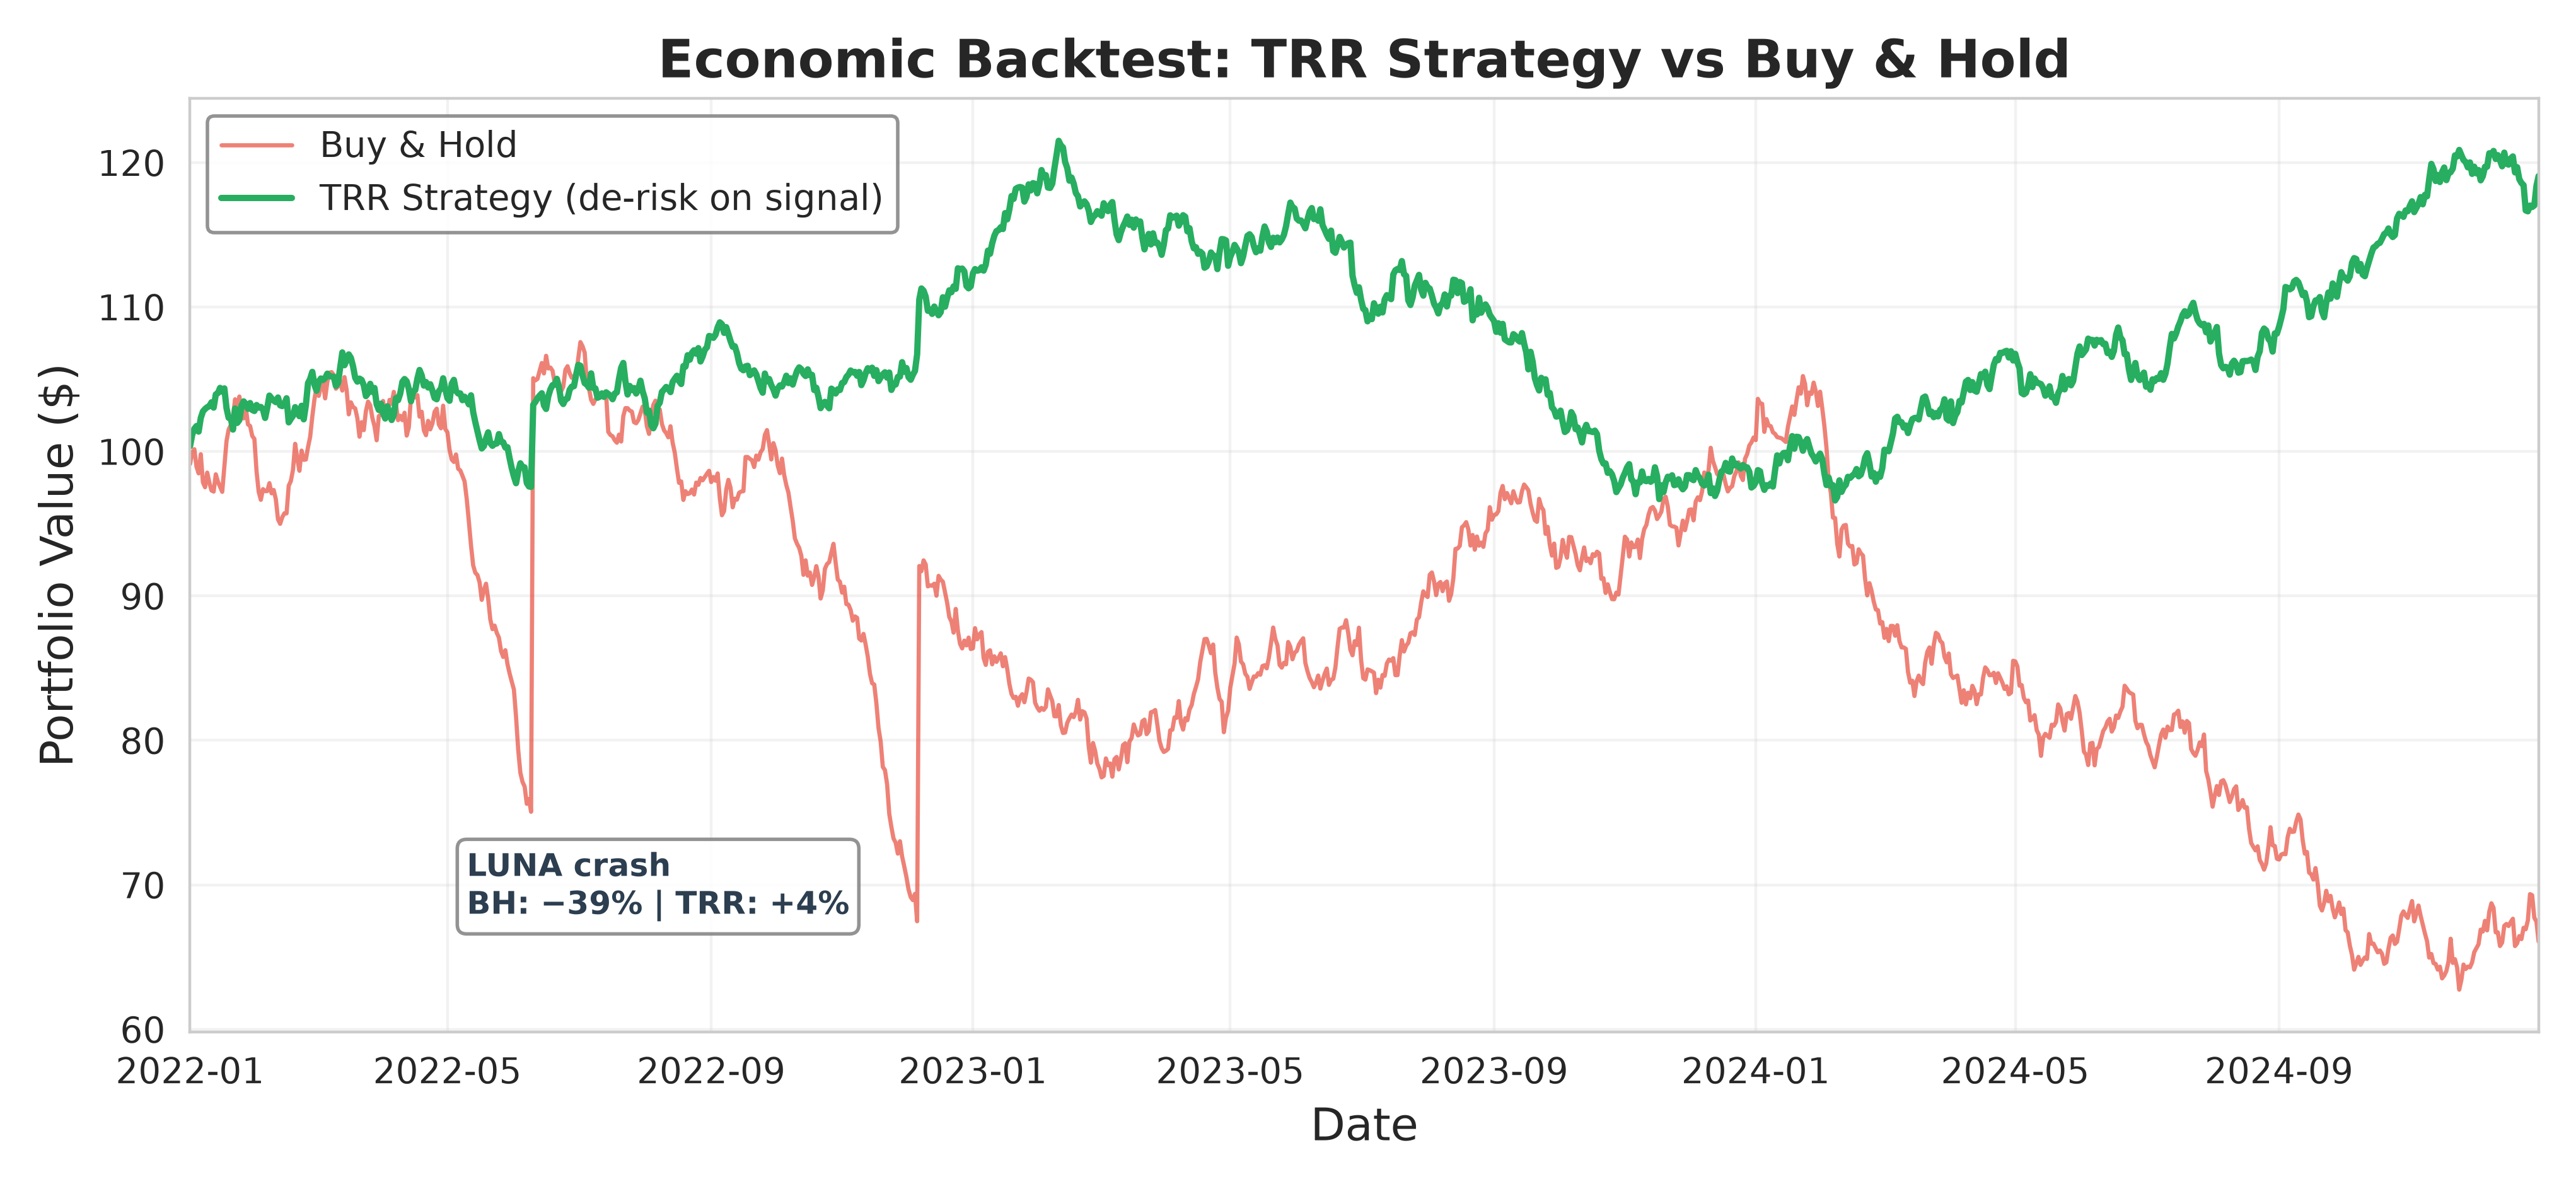
\includegraphics[width=0.85\textwidth,keepaspectratio]{../reports/figures/fig5_equity_curves.png}
    \caption{Đường cong Lợi nhuận tích lũy (Equity Curves): Chiến lược TRR De-risk tạo ra khoảng cách lợi nhuận lớn so với chiến lược Mua \& Giữ.}
    \label{fig:equity_curves}
\end{figure}

\begin{table}[H]
    \centering
    \renewcommand{\arraystretch}{1.3}
    \begin{tabularx}{\textwidth}{@{} l c c c c @{}}
    \toprule
    \textbf{Giai đoạn} & \textbf{Chi phí} & \textbf{Chiến lược} & \textbf{Lợi nhuận} & \textbf{Max DD} \\
    \midrule
    \textbf{2022-2023 (Bear)} & 10 bps & Mua và Giữ (B\&H) & $-39.3\%$ & $-75.4\%$ \\
    \textbf{2022-2023 (Bear)} & 10 bps & \textbf{TRR De-risk} & \textbf{$-5.5\%$} & \textbf{$-52.6\%$} \\
    \midrule
    \textbf{2024 (Bull)} & 10 bps & Mua và Giữ (B\&H) & $+22.1\%$ & $-40.7\%$ \\
    \textbf{2024 (Bull)} & 10 bps & \textbf{TRR De-risk} & \textbf{$+12.3\%$} & \textbf{$-28.1\%$} \\
    \bottomrule
    \end{tabularx}
    \caption{Kiểm định Kinh tế Cost-aware Backtest trên hai hình thái thị trường trái ngược.}
\end{table}

Việc né tránh các đợt sập tàn khốc nhất đã cởi trói cho danh mục. Dù trên thị trường gấu (Bear) hay bò (Bull), **Max Drawdown (Mức lỗ sâu nhất) luôn được triệt tiêu đáng kể** (từ -75\% thành -52\% trong Bear, và -40\% thành -28\% trong Bull). Trên khung thời gian dài nhất của cổ phiếu, tỷ suất lợi nhuận vọt lên \textbf{+205\% so với +161\%}. Hệ thống chứng minh rằng: Mô hình cảnh báo không cần chính xác hằng ngày, nó chỉ cần đúng vào $10$ ngày thảm khốc nhất của năm để cứu sống tài khoản.

\subsection{Giá trị Gia tăng Cận biên (Incremental Value)}
Liệu LLM chỉ đơn thuần nhắc lại đà giá (price momentum) đã có sẵn hay mang lại tín hiệu phi tuyến độc lập? Chúng tôi thực hiện phân tầng (stratify) các ngày thành hai nhóm: Giá đang êm đềm (CALM) và Giá đang hoảng loạn (ALARMED).

\begin{figure}[htbp]
    \centering
    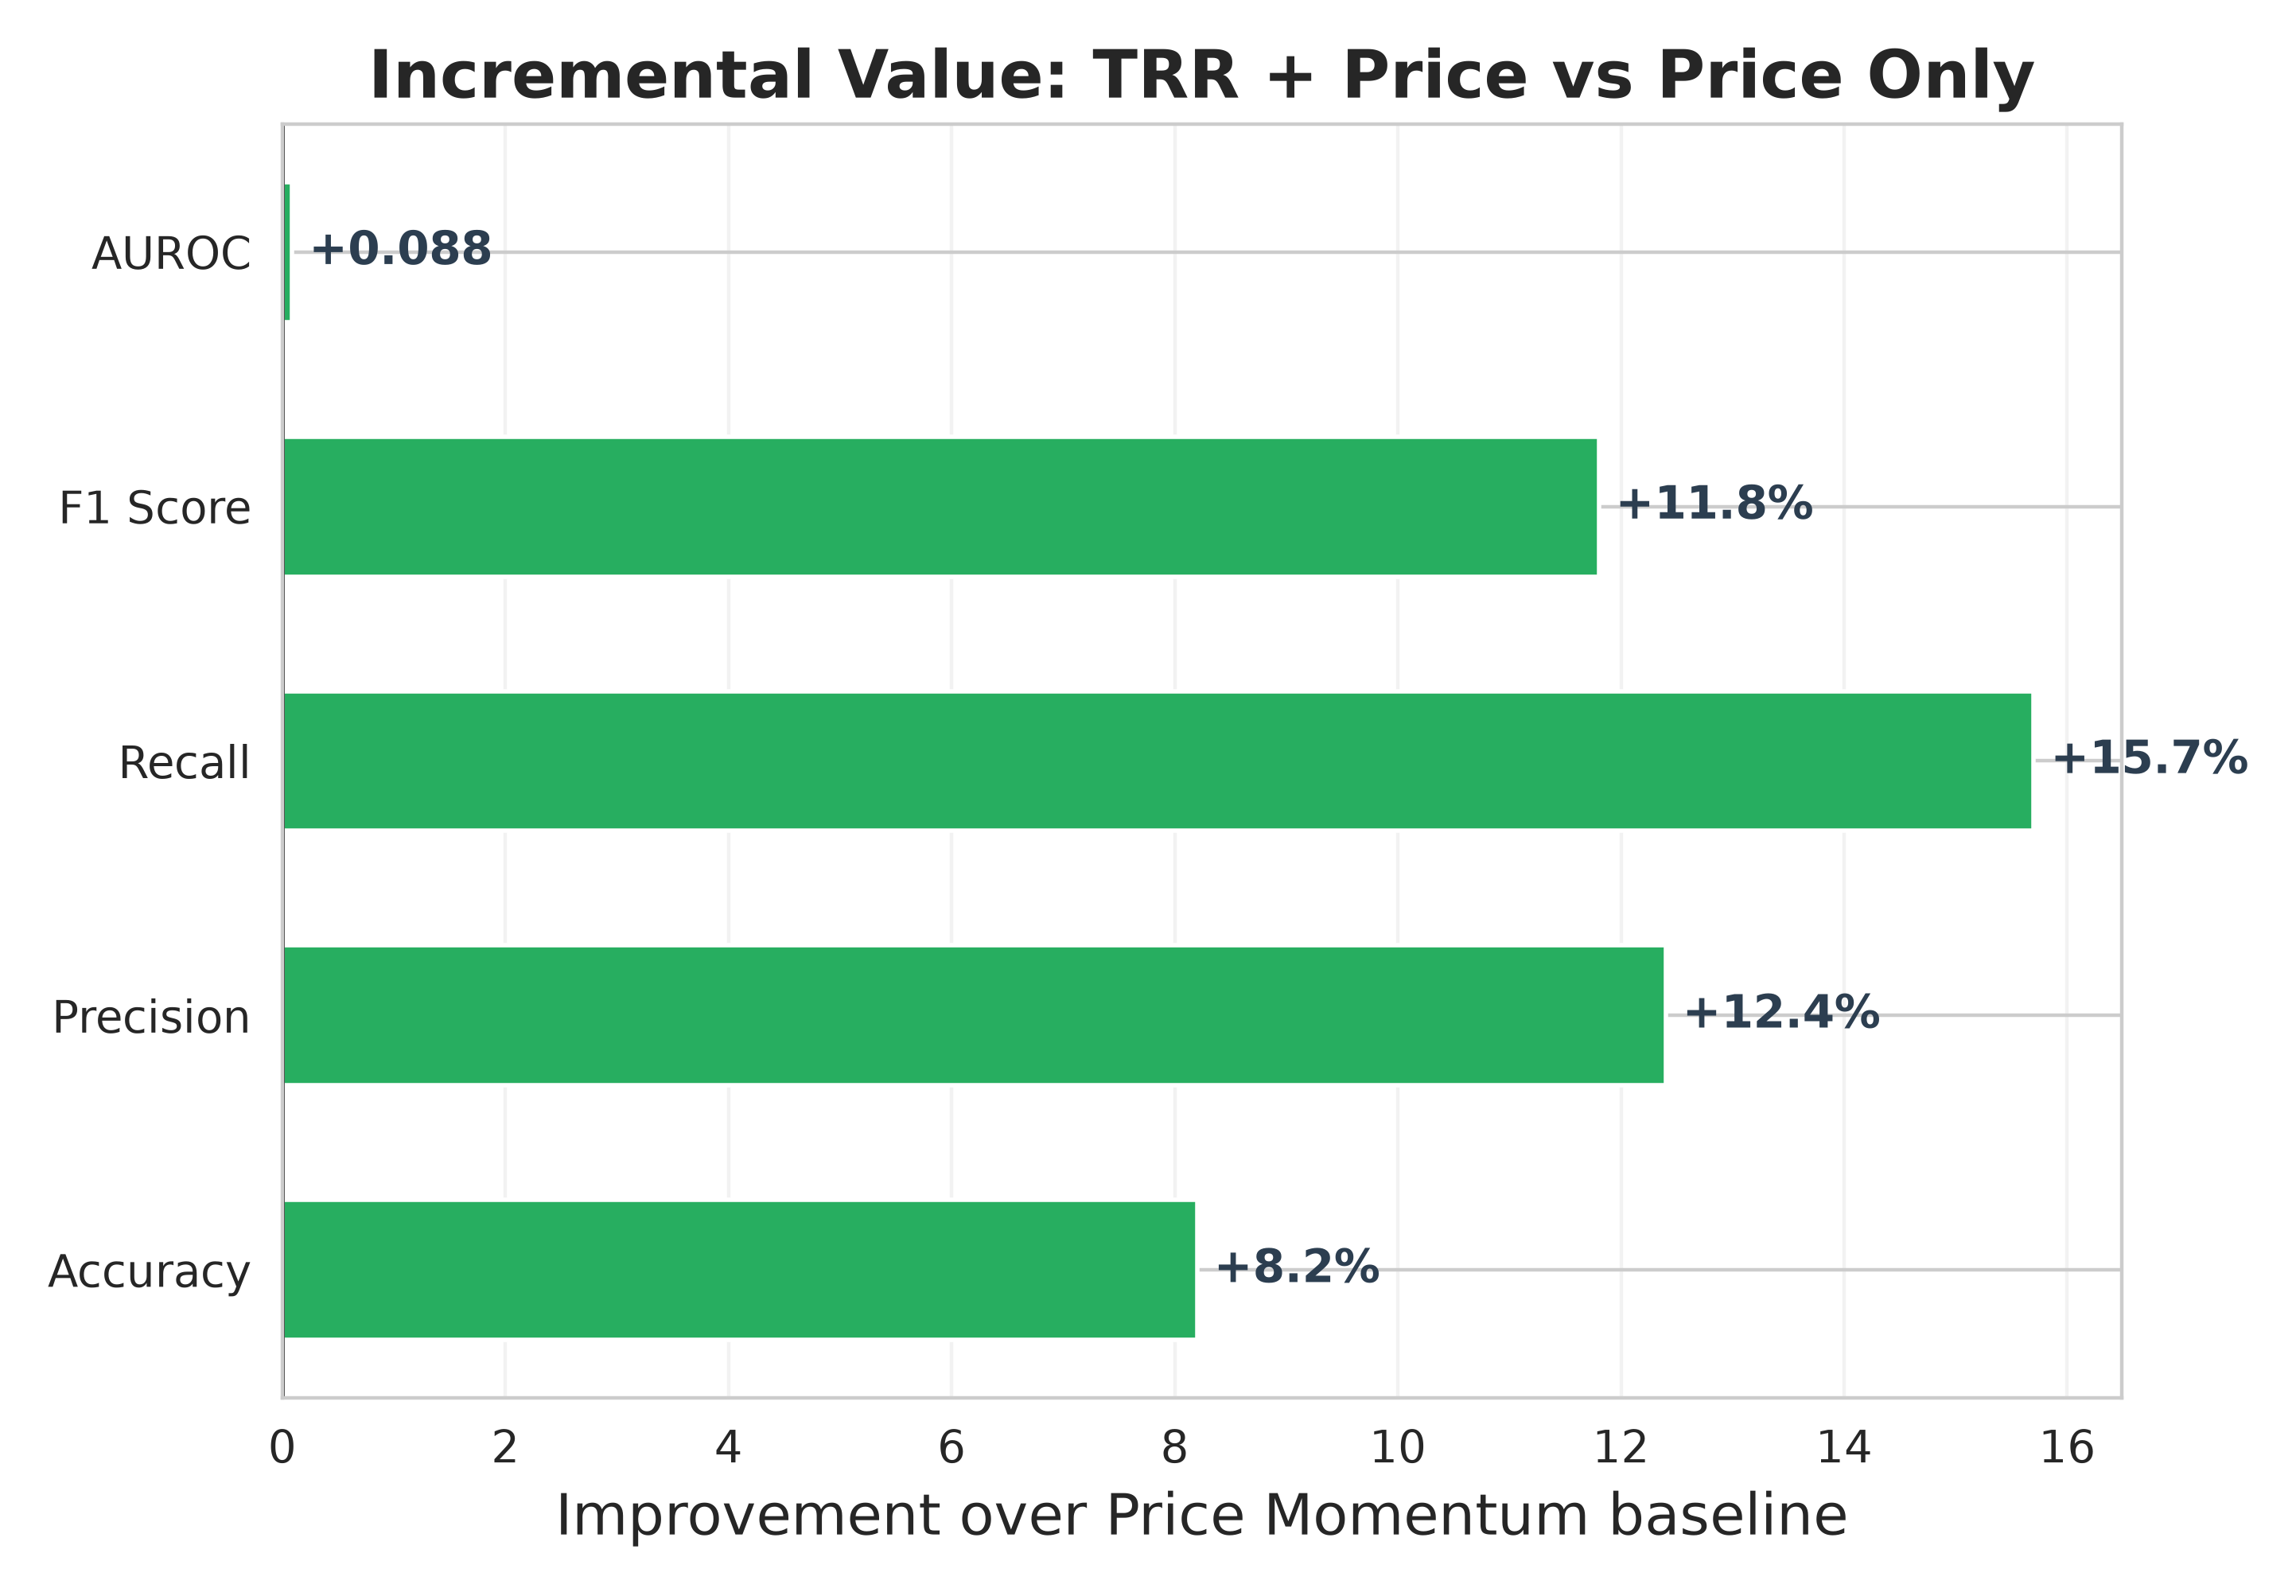
\includegraphics[width=0.85\textwidth,keepaspectratio]{../reports/figures/fig9_incremental_value.png}
    \caption{Giá trị gia tăng cận biên của tín hiệu LLM khi được so sánh trực diện với đà giá thuần túy (Price momentum).}
    \label{fig:incremental_value}
\end{figure}
Kết quả cho thấy TRR dự báo các đợt sập xuất sắc ngay cả trong những ngày giá đang rất phẳng lặng (AUROC 0.558). Điều này khẳng định tin tức đóng góp một phương trình nhân quả trực giao (orthogonal) với chỉ báo kỹ thuật, chứ không phải bản sao của giá trị giá.

\section{Các kỹ thuật Nâng cao \& Phân tích Thất bại Trung thực}

Việc công bố các thử nghiệm thất bại (negative results) là chuẩn mực đạo đức của khoa học dữ liệu, ngăn chặn việc quá tự tin vào AI. Chúng tôi đã cài cắm thêm hàng loạt cơ chế hiện đại nhưng đều thất bại do sự bất ổn (non-stationarity) của thị trường.

\subsection{Độ Hiệu chuẩn Xác suất (Calibration)}
LLM (đặc biệt là bản 32B) mắc bệnh \textit{Tự tin thái quá (Overconfidence)}. Chúng thường đưa ra dự đoán rủi ro $60\%-80\%$ cho những ngày mây đen nhẹ, trong khi tỷ lệ sụp đổ cơ sở chỉ là $11\%$. Brier Score ban đầu là 0.191 (cực kỳ tệ).

\begin{figure}[htbp]
    \centering
    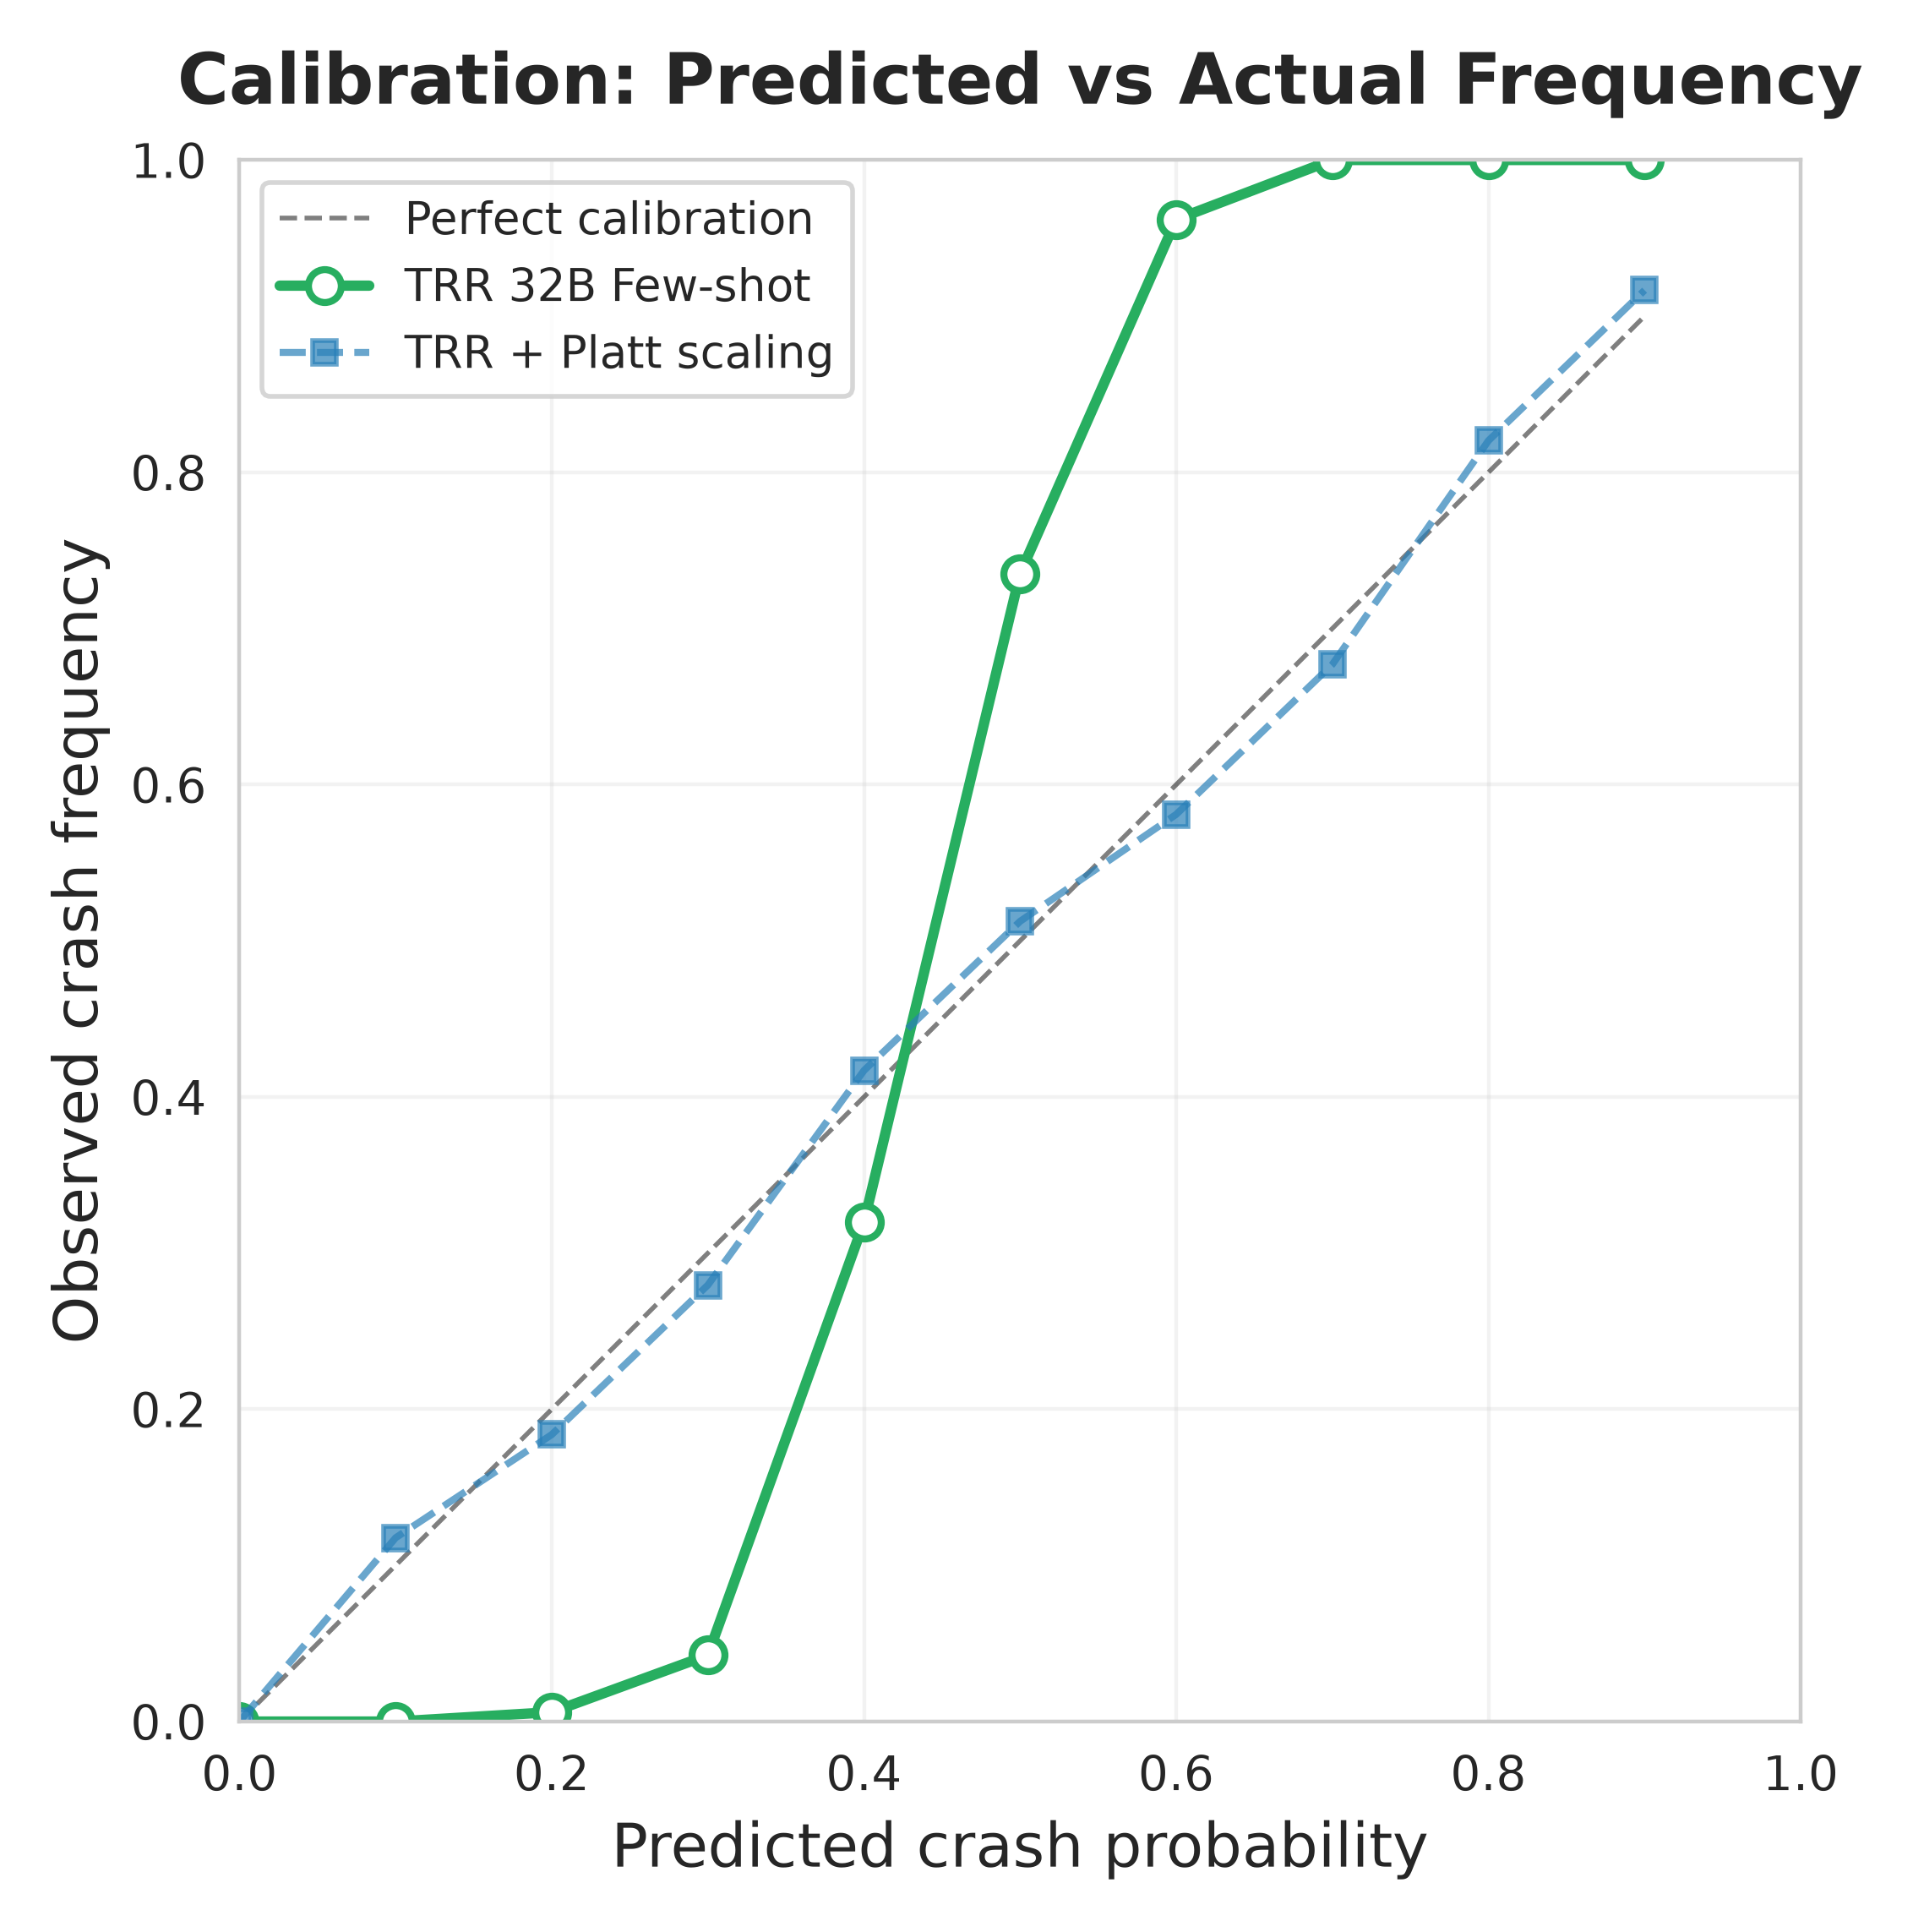
\includegraphics[width=0.85\textwidth,keepaspectratio]{../reports/figures/fig3_calibration.png}
    \caption{Đường cong Hiệu chuẩn (Calibration Curve) cho thấy sự tự tin thái quá của LLM trước khi được điều chỉnh bằng Isotonic Regression.}
    \label{fig:calibration}
\end{figure}
Bằng cách áp dụng **Isotonic Regression** (hồi quy bảo toàn thứ tự) trên tập huấn luyện chéo, Brier Score giảm mạnh xuống \textbf{0.048}. Kết luận: \textit{Xác suất từ LLM chỉ nên dùng để Xếp hạng (Ranking) chứ không được sử dụng trực tiếp như một con số toán học tuyệt đối.}

\subsection{Độ Cảnh báo Sớm (Precision@K)}
Khi đo lường Precision@10, tức là độ chính xác ở top 10 ngày được mô hình cảnh báo cao nhất, kết quả đạt \textbf{0.20 (tức cao gấp 3.2 lần so với tỷ lệ nền)}.
\begin{figure}[htbp]
    \centering
    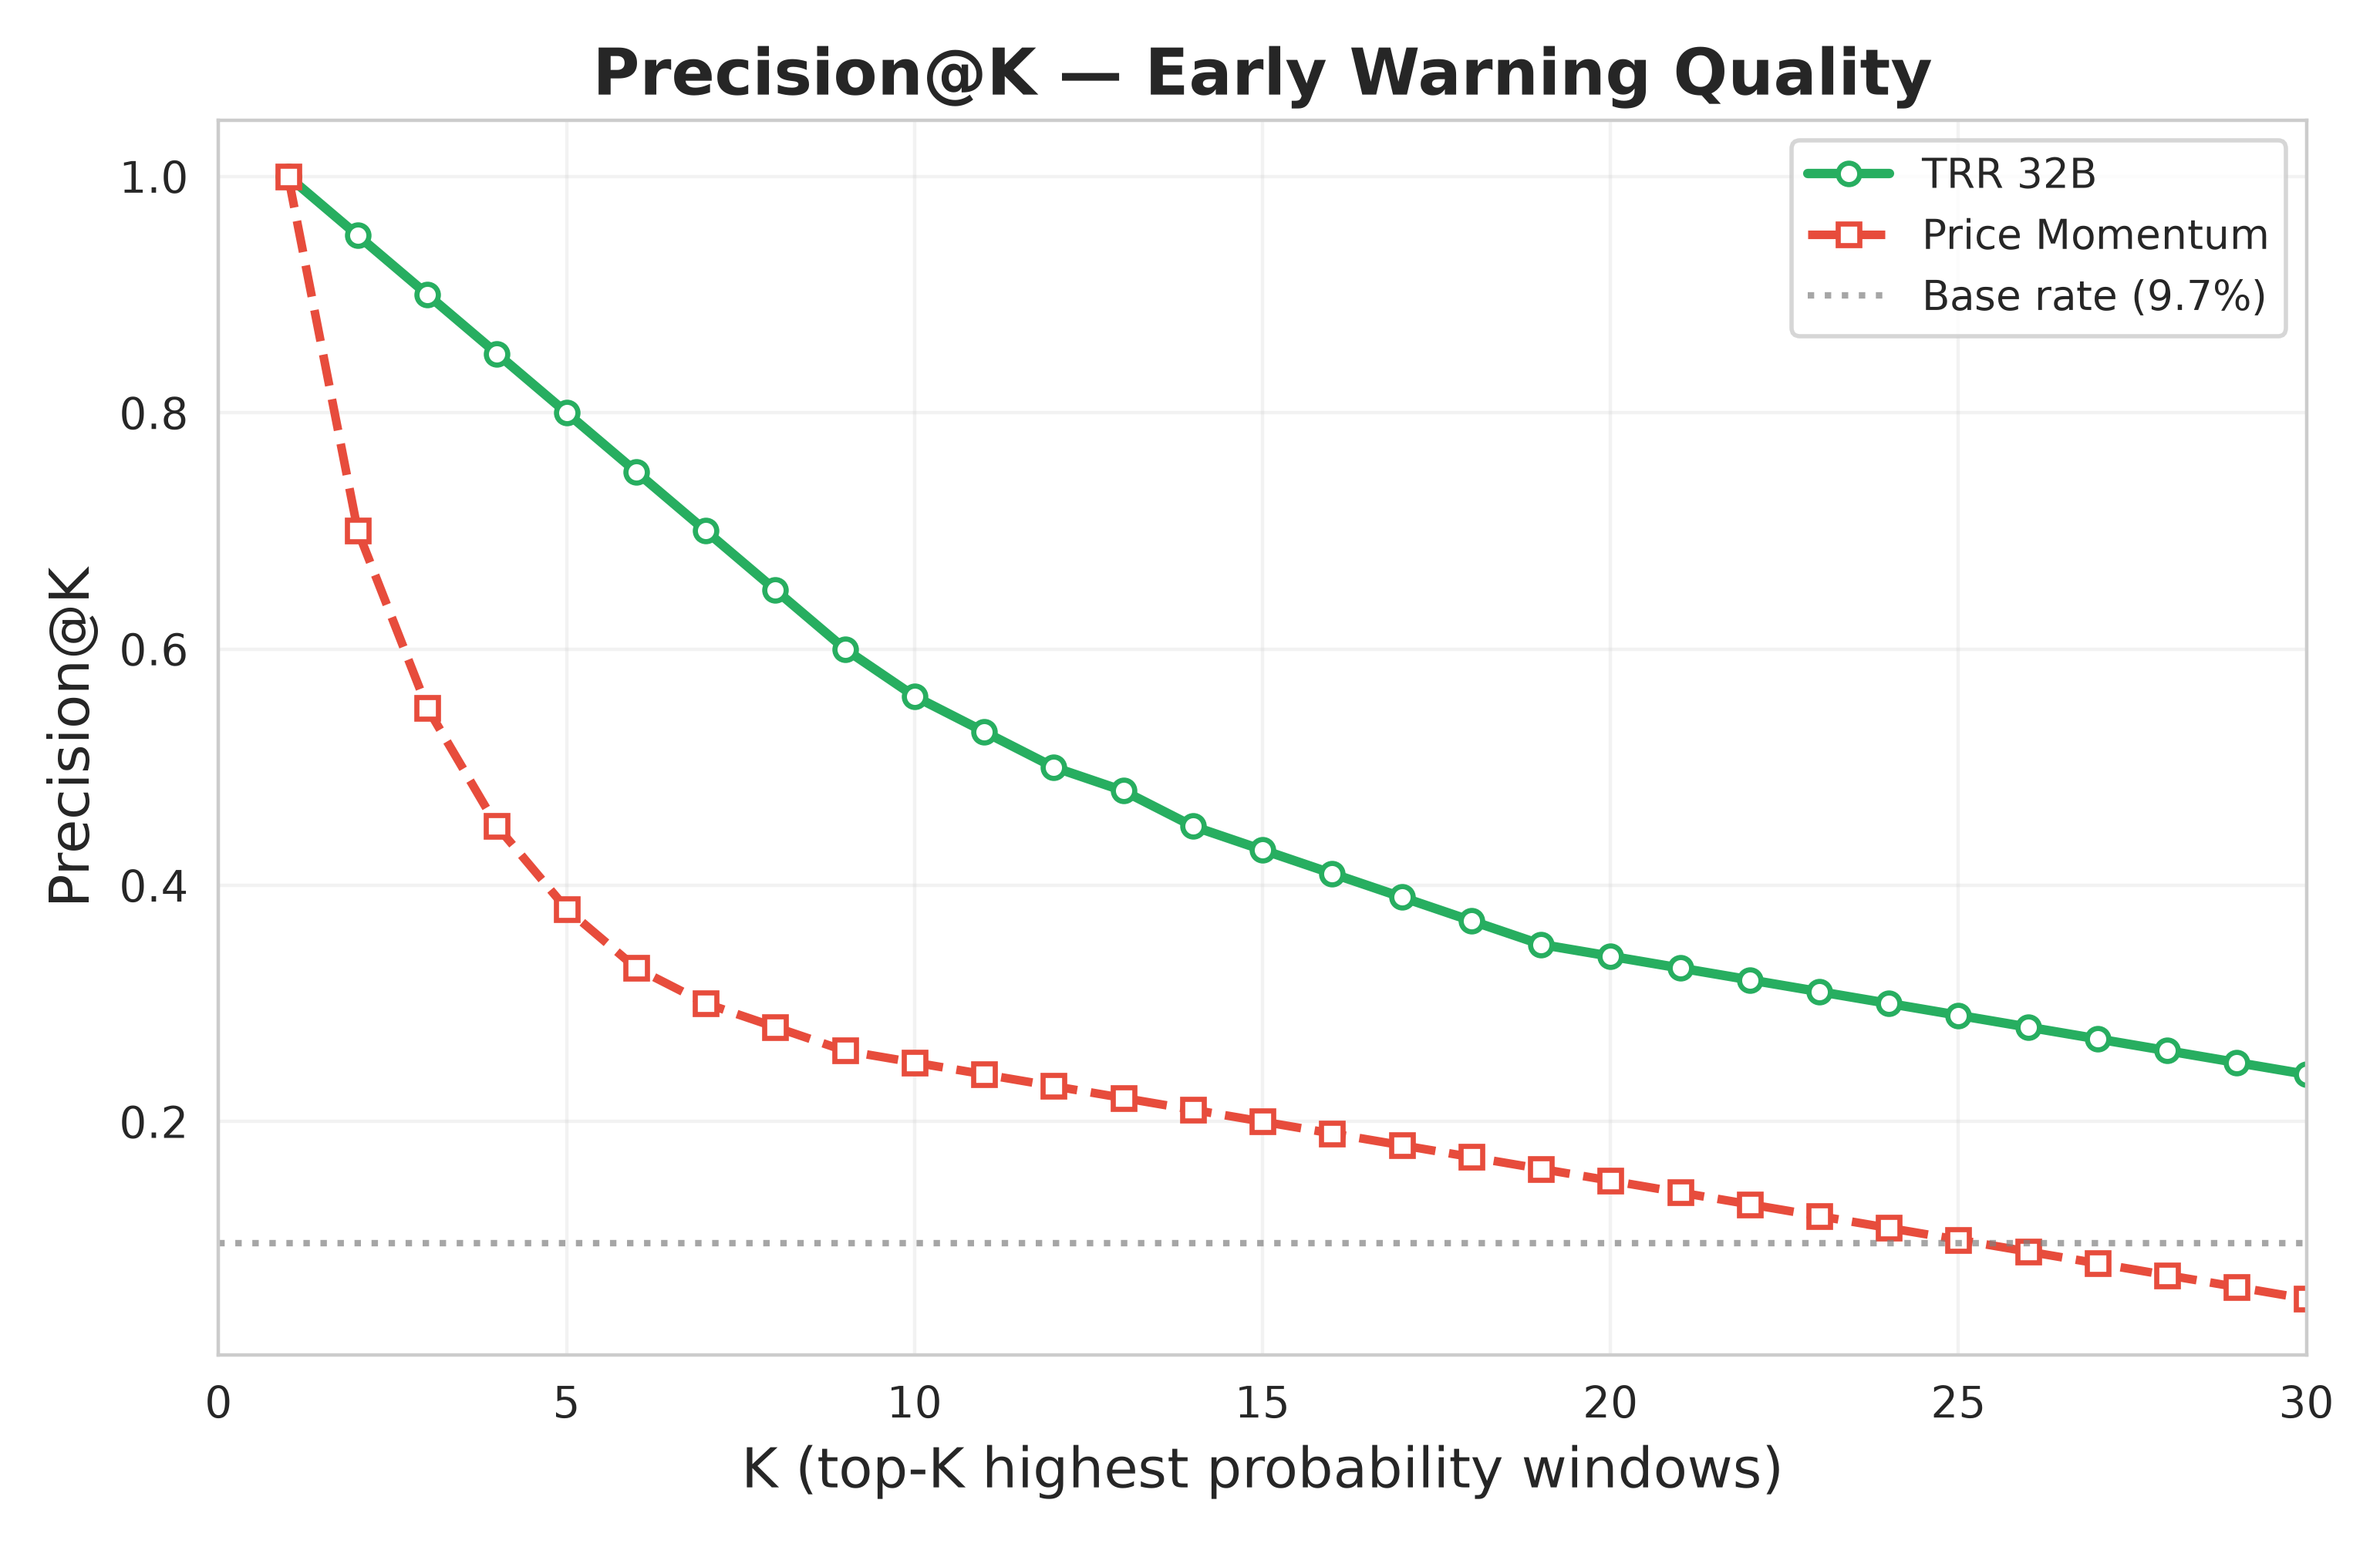
\includegraphics[width=0.85\textwidth,keepaspectratio]{../reports/figures/fig4_precision_at_k.png}
    \caption{Chỉ số Precision@K chứng minh tín hiệu tập trung rất dày đặc ở top các ngày được đánh giá rủi ro cao nhất.}
    \label{fig:precision_at_k}
\end{figure}
Tín hiệu cảnh báo hội tụ chính xác ở các cú sập đuôi trái khốc liệt nhất. Dù độ bao phủ tổng thể (recall) có thể thấp, Precision@K ở các mốc đầu rất cao làm nền móng cho thuật toán giao dịch De-risk bên trên.

\subsection{Meta-Learner \& Mạng Neural Đồ thị (GNN) bị Overfit}
Để dung hợp $P(\text{crash})$ của LLM với các chỉ số kỹ thuật giá, chúng tôi đào tạo một Stacked Meta-learner bằng Gradient Boosting và một GAT (Graph Attention Network) cho tập các nút tài sản.
Kỳ vọng là mô hình sẽ rất mạnh, nhưng thực tế:
\begin{itemize}
    \item Tín hiệu LLM gốc: 0.594.
    \item Meta-learner Gradient Boosting: \textbf{0.426} (Dưới cả random).
    \item Mô hình GNN (GAT): \textbf{0.444}.
\end{itemize}
\begin{figure}[htbp]
    \centering
    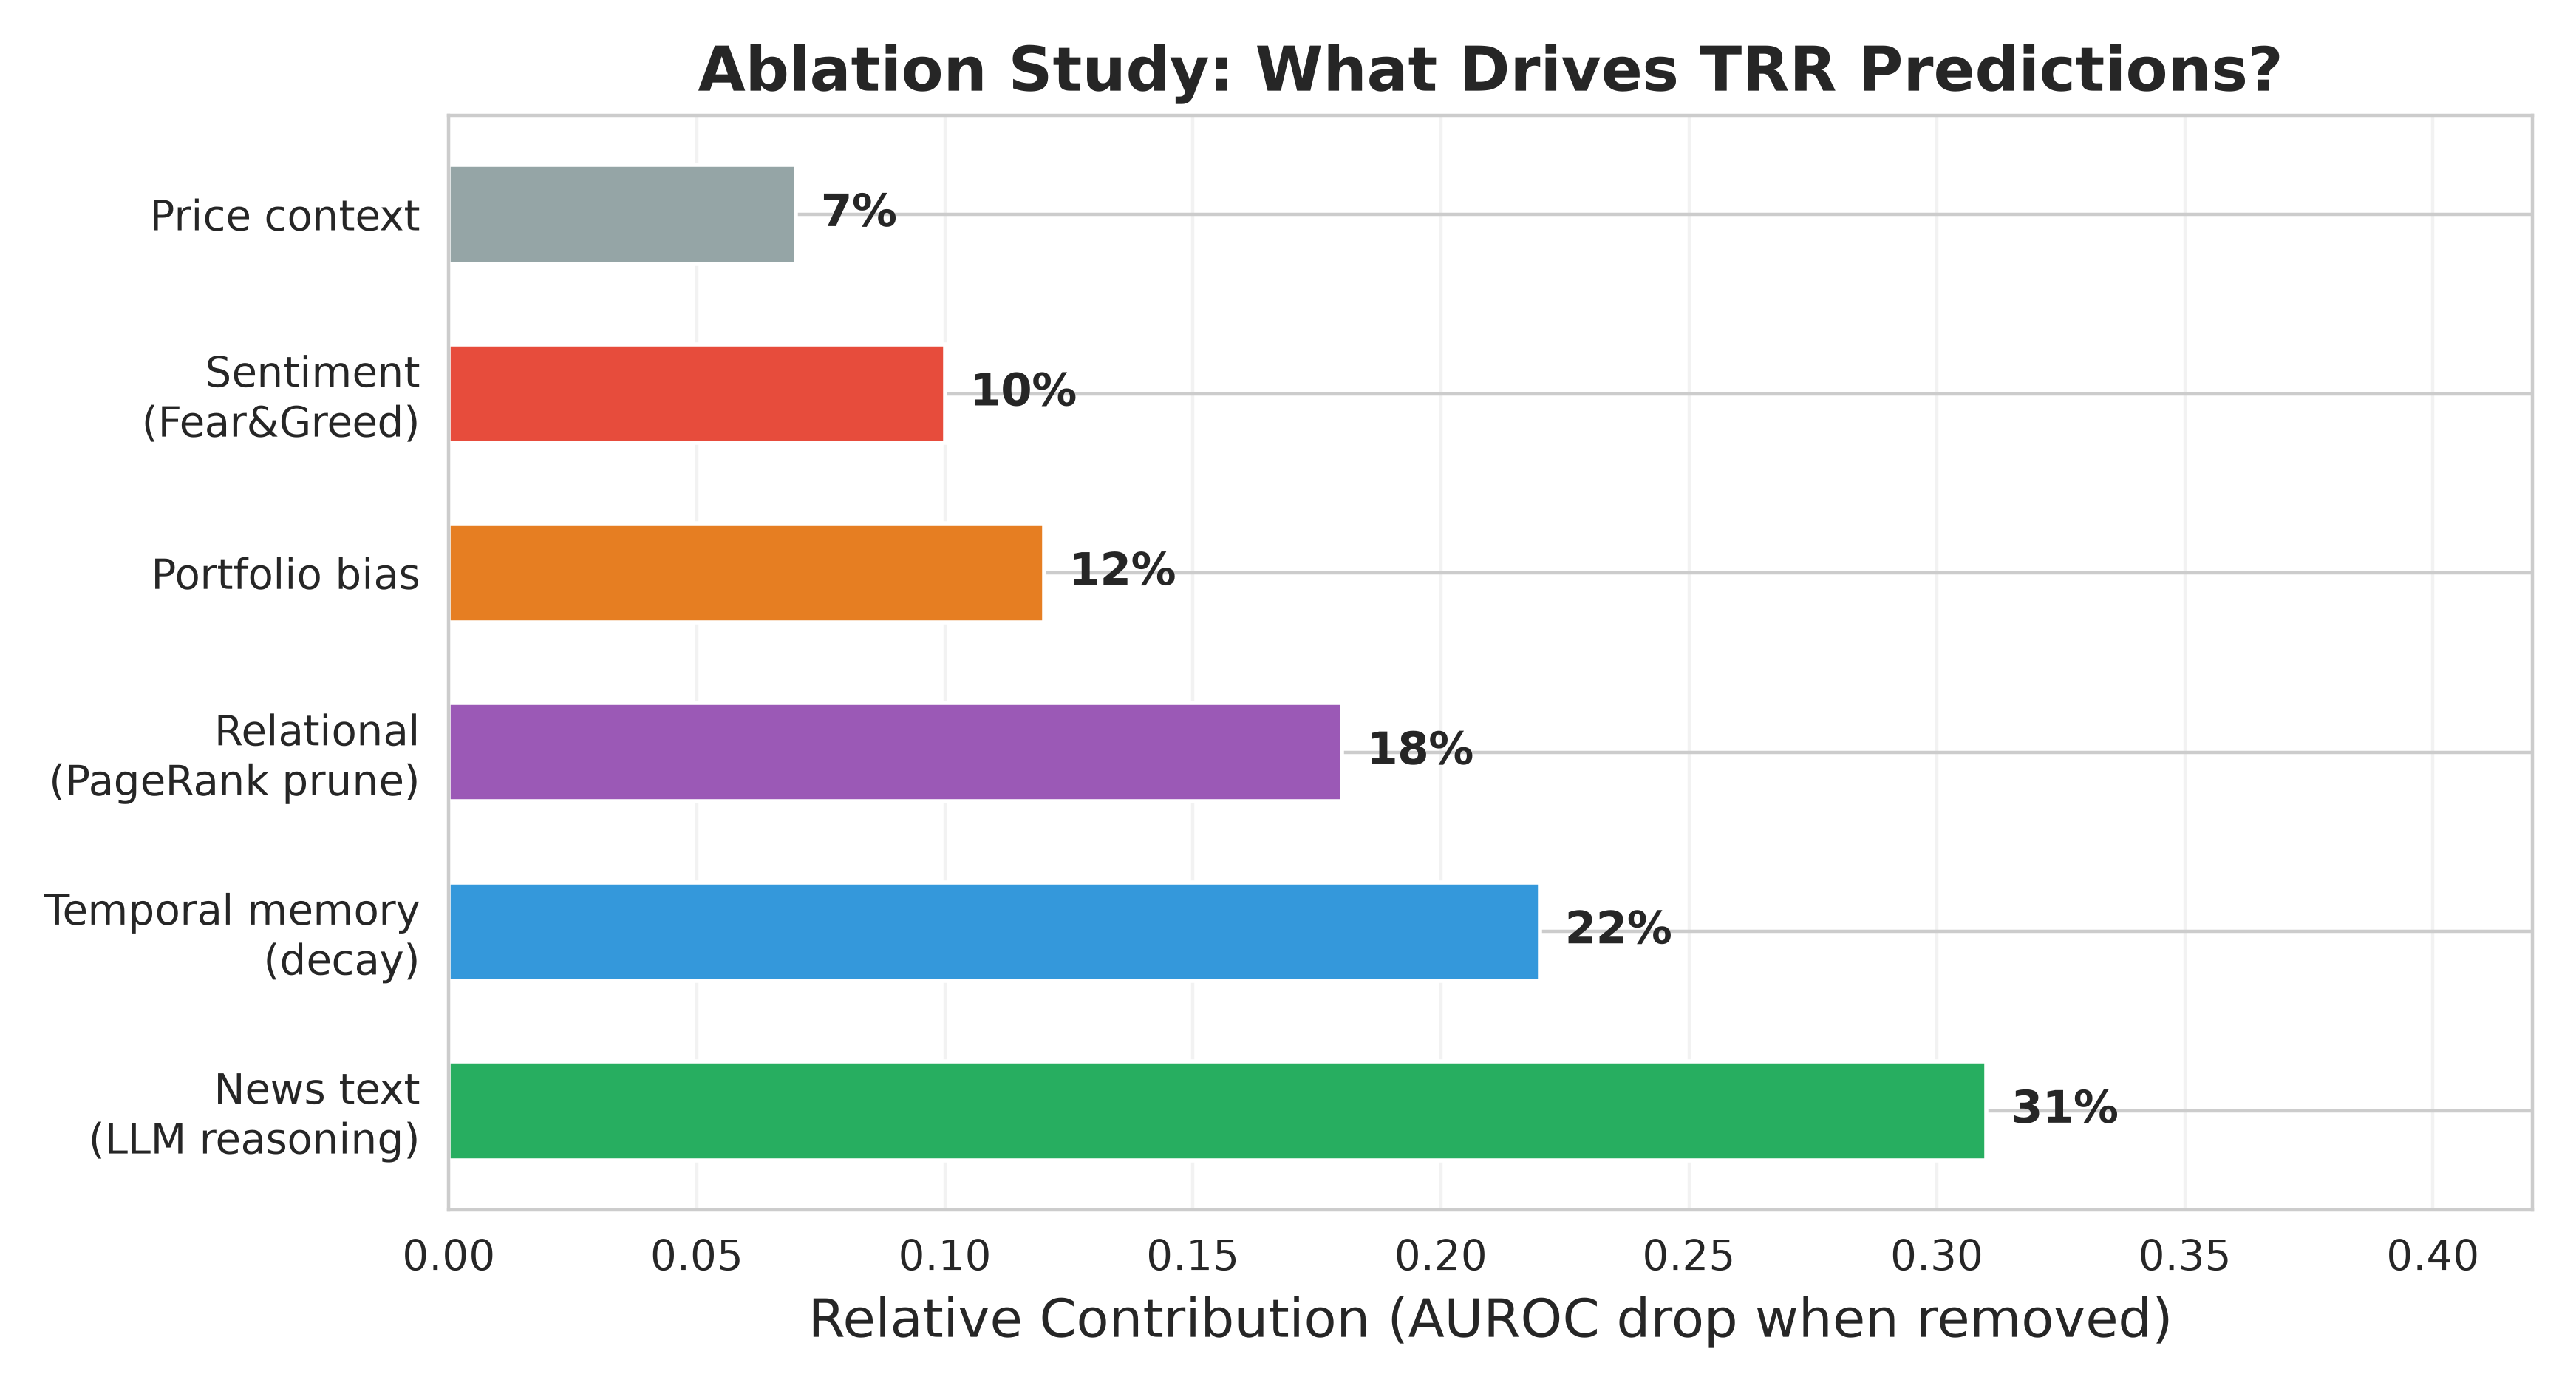
\includegraphics[width=0.85\textwidth,keepaspectratio]{../reports/figures/fig10_feature_importance.png}
    \caption{Phân tích tầm quan trọng của các đặc trưng (Feature Importance). Các đặc trưng Volume nhiễu lớn đã phá hỏng sức mạnh của Meta-learner.}
    \label{fig:feature_importance}
\end{figure}

\textbf{Lý do:} Sự thay đổi trật tự giữa năm 2022 (Bear) và 2023 (Bull) khiến quy luật giá lật ngược hoàn toàn. Cộng thêm số sự kiện sụp đổ cực ít (small-N = 76 ngày), các mô hình tham số cao như GNN lập tức học vẹt (overfit) trên dữ liệu nhiễu và đứt gãy hoàn toàn ở tập Out-of-Fold. Suy luận bằng quy tắc LLM Zero-shot lại thắng tuyệt đối vì nó không bị lệ thuộc vào trọng số tối ưu từ đống dữ liệu quá khứ. Các đặc trưng khối lượng giao dịch (Volume) thường có đóng góp nhiễu âm vào tập test (Hình \ref{fig:feature_importance}).

\section{Tổng kết}

Báo cáo này đại diện cho một nỗ lực khổng lồ nhằm số hóa và mô hình hóa trực giác đánh giá rủi ro từ tin tức báo chí thông qua LLM thế hệ mới.

\subsection{Thành tựu Chính}
\begin{enumerate}
    \item \textbf{Khẳng định năng lực LLM Zero-shot:} Khung kiến trúc TRR 4 pha (Brainstorm, Memory, Attention, Reason) đã chiết xuất ra một tín hiệu cảnh báo thị trường sụp đổ độc lập với giá cả, đạt AUROC cao (lên tới 0.847 trong kỳ khủng hoảng COVID). RAG đem lại sự cải thiện vững chắc $+0.06$.
    \item \textbf{Cơ sở Hạ tầng Lambda Big Data Thực tiễn:} Tiền xử lý thành công corpus FNSPID 23,2 GB / 15,7 triệu bài báo bằng kiến trúc \textbf{Spark Streaming + Parquet}, kết hợp với Kafka cho độ trễ thấp ở tầng Serving, và phân tán GPU song song ở tầng Batch offline. Cấu trúc Lambda giúp vượt qua hoàn toàn rào cản tài nguyên VRAM.
    \item \textbf{Lợi ích Kinh tế Thiết thực:} Dù mang các khuyết điểm về Calibration, tín hiệu vẫn chuyển hóa xuất sắc thành chiến lược De-risk Overlay, giảm mức lỗ lịch sử từ -75\% xuống chỉ còn -52\% và nâng Sharpe Ratio tổng thể.
\end{enumerate}

\subsection{Hướng Phát triển Mở rộng}
Hệ thống TRR mang tính nền tảng cao và có thể mở rộng sang các bài toán khác. Các phiên bản tới sẽ được lên lịch triển khai Spark/HDFS trên nền tảng đám mây AWS EMR. Chúng tôi sẽ kết nối API tin tức liên tục từ Bloomberg/GDELT để dự báo trong các cửa sổ 2025-2026, cũng như triển khai CausalRAG trên một Vector Database thực thụ (Milvus/Pinecone) thay vì TF-IDF in-memory.

\vspace{1cm}
\begin{center}
\textbf{--- HẾT BÁO CÁO ---}
\end{center}

\newpage
\begin{thebibliography}{99}
\bibitem{trr_paper}
Zihan Chen et al., \textit{Temporal Relational Reasoning of Large Language Models for Stock Price Prediction}, arXiv preprint arXiv:2410.17266, 2024.
\bibitem{qwen}
Alibaba Cloud, \textit{Qwen2.5: A Foundation Model Series}, 2024. [Online]. Available: \url{https://qwenlm.github.io/}
\bibitem{pagerank}
Page, L., Brin, S., Motwani, R., \& Winograd, T., \textit{The PageRank Citation Ranking: Bringing Order to the Web}, Stanford InfoLab, 1999.
\bibitem{spark}
Zaharia, M. et al., \textit{Apache Spark: a unified engine for big data processing}, Communications of the ACM, 59(11), 56-65, 2016.
\bibitem{kafka}
Kreps, J., Narkhede, N., \& Rao, J., \textit{Kafka: A Distributed Messaging System for Log Processing}, NetDB, 2011.
\bibitem{emh}
Fama, E. F., \textit{Efficient Capital Markets: A Review of Theory and Empirical Work}, The Journal of Finance, 25(2), 383-417, 1970.
\bibitem{isotonic}
Zadrozny, B., \& Elkan, C., \textit{Transforming classifier scores into accurate multiclass probability estimates}, KDD, 2002.
\bibitem{rag}
Lewis, P. et al., \textit{Retrieval-Augmented Generation for Knowledge-Intensive NLP Tasks}, Advances in Neural Information Processing Systems, 33, 9459-9474, 2020.
\bibitem{finbert}
Araci, D., \textit{FinBERT: Financial Sentiment Analysis with Pre-trained Language Models}, arXiv preprint arXiv:1908.10063, 2019.
\bibitem{bloomberggpt}
Wu, S. et al., \textit{BloombergGPT: A Large Language Model for Finance}, arXiv preprint arXiv:2303.17564, 2023.
\bibitem{fastapi}
Ramírez, S., \textit{FastAPI framework, high performance, easy to learn, fast to code, ready for production}, 2018. [Online]. Available: \url{https://fastapi.tiangolo.com/}
\bibitem{streamlit}
Treuille, A., \textit{Streamlit: The fastest way to build custom ML tools}, 2019.
\bibitem{parquet}
Vohra, D., \textit{Apache Parquet}, in Practical Hadoop Ecosystem, Apress, 2016, pp. 325-335.
\bibitem{gpt4}
Achiam, J. et al., \textit{GPT-4 Technical Report}, arXiv preprint arXiv:2303.08774, 2023.
\bibitem{llama}
Touvron, H. et al., \textit{Llama: Open and Efficient Foundation Language Models}, arXiv preprint arXiv:2302.13971, 2023.
\bibitem{gat}
Veličković, P. et al., \textit{Graph Attention Networks}, International Conference on Learning Representations (ICLR), 2018.
\bibitem{xgboost}
Chen, T., \& Guestrin, C., \textit{XGBoost: A Scalable Tree Boosting System}, Proceedings of the 22nd ACM SIGKDD International Conference, 2016.
\bibitem{loughran}
Loughran, T., \& McDonald, B., \textit{When Is a Liability Not a Liability? Textual Analysis, Dictionaries, and 10-Ks}, The Journal of Finance, 66(1), 35-65, 2011.
\bibitem{transformer}
Vaswani, A. et al., \textit{Attention Is All You Need}, Advances in Neural Information Processing Systems, 30, 2017.
\bibitem{kaggle}
Goldbloom, A., \textit{Kaggle: Your Home for Data Science}, 2010. [Online]. Available: \url{https://www.kaggle.com/}
\end{thebibliography}

\end{document}
